\chapter{Experiments and Results}

\section{Datasets}

This section describes the data used to evaluate the proposed method. We outline the selected benchmark dataset, the specific scenes considered, and the properties that make them suitable for assessing geometry-aware regularization.

\subsection{Deep Blending Dataset}

We evaluate the proposed method on the Deep Blending dataset~\cite{hedman2018deepblending}, which is widely used in neural rendering research for benchmarking view synthesis and reconstruction quality. The dataset consists of multi-view image sequences with accurately estimated camera poses obtained through Structure-from-Motion pipelines using COLMAP~\cite{schoenberger2016sfm}.

We focus on three indoor scenes from the Deep Blending dataset: \textbf{DrJohnson}, \textbf{Library}, and \textbf{Playroom}. These scenes are characterized by challenging indoor environments with large planar regions, reflective surfaces, and areas with limited texture. Indoor environments are particularly suitable for evaluating geometry-aware priors because they contain dominant planar structures (walls, floors, ceilings, furniture surfaces) that benefit significantly from structural regularization. All quantitative results reported in this chapter represent averages computed across these three scenes unless otherwise specified.

\begin{figure}[h]
    \centering
    \begin{subfigure}{0.32\textwidth}
        \centering
        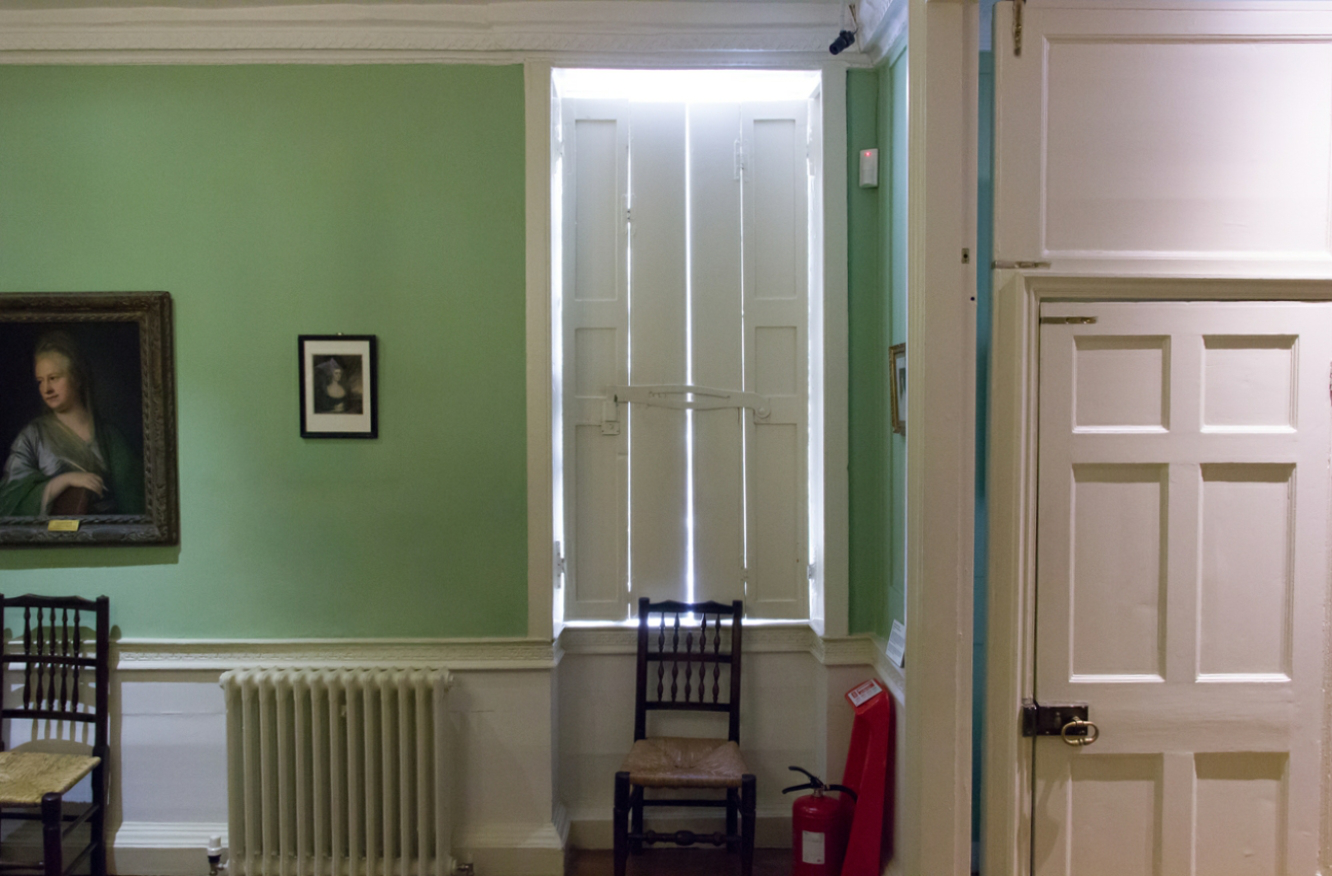
\includegraphics[width=\textwidth]{comparison_figures/drjohnson_gt_view01.png}
        \caption{DrJohnson: green room}
    \end{subfigure}
    \hfill
    \begin{subfigure}{0.32\textwidth}
        \centering
        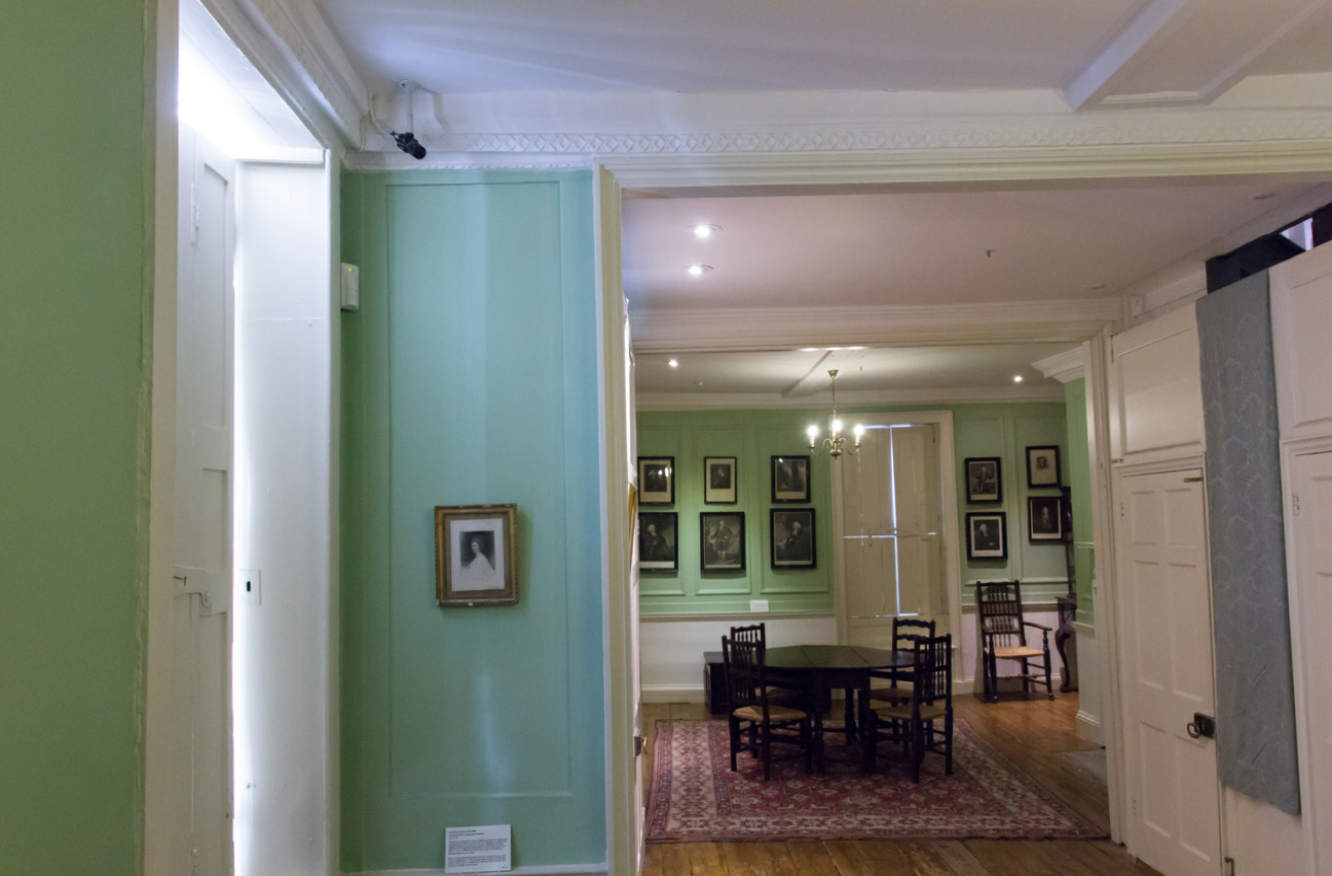
\includegraphics[width=\textwidth]{comparison_figures/drjohnson_gt_view03.png}
        \caption{DrJohnson: hallway}
    \end{subfigure}
    \hfill
    \begin{subfigure}{0.32\textwidth}
        \centering
        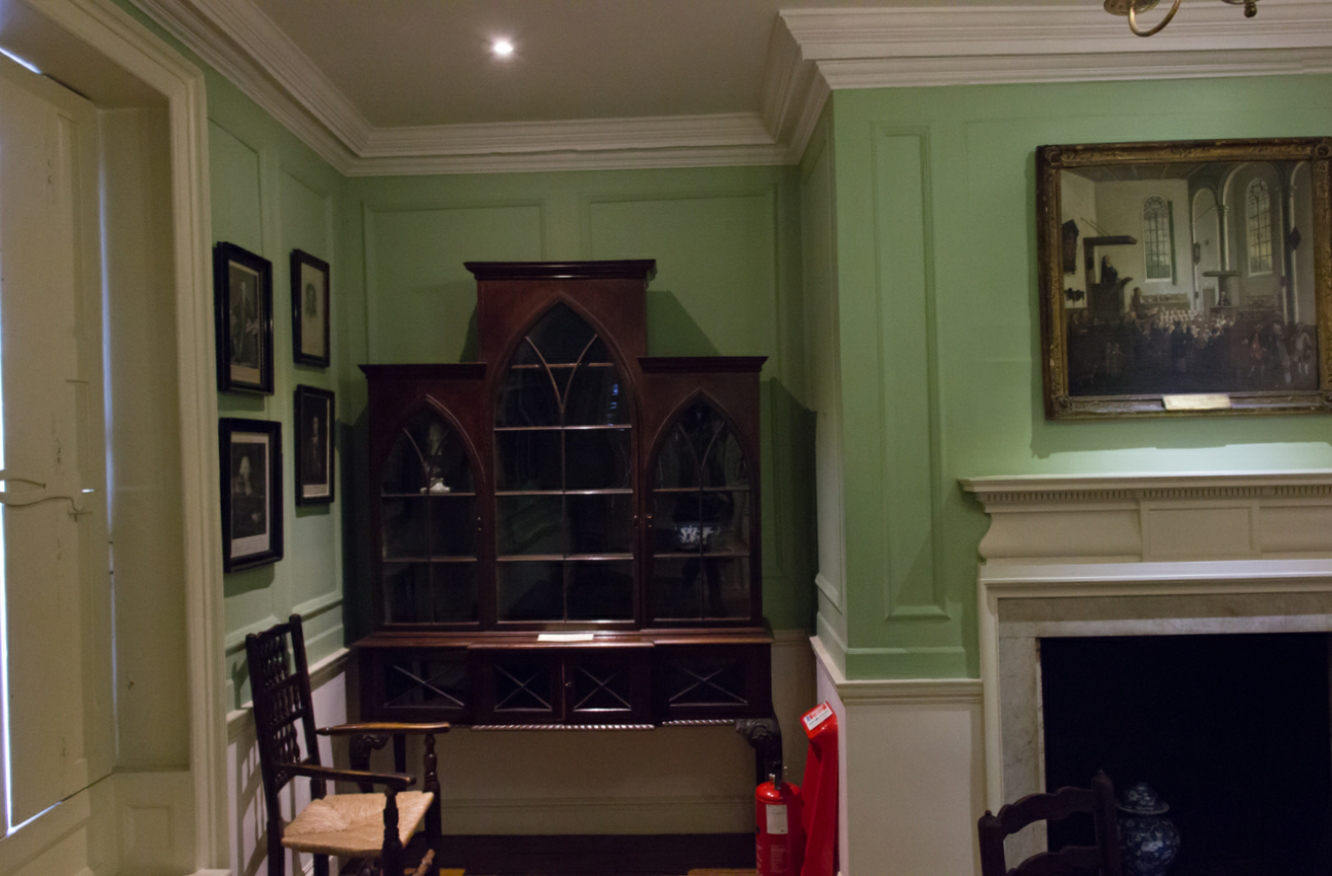
\includegraphics[width=\textwidth]{comparison_figures/drjohnson_gt_view04.png}
        \caption{DrJohnson: cabinet room}
    \end{subfigure}

    \vspace{0.5em}

    \begin{subfigure}{0.48\textwidth}
        \centering
        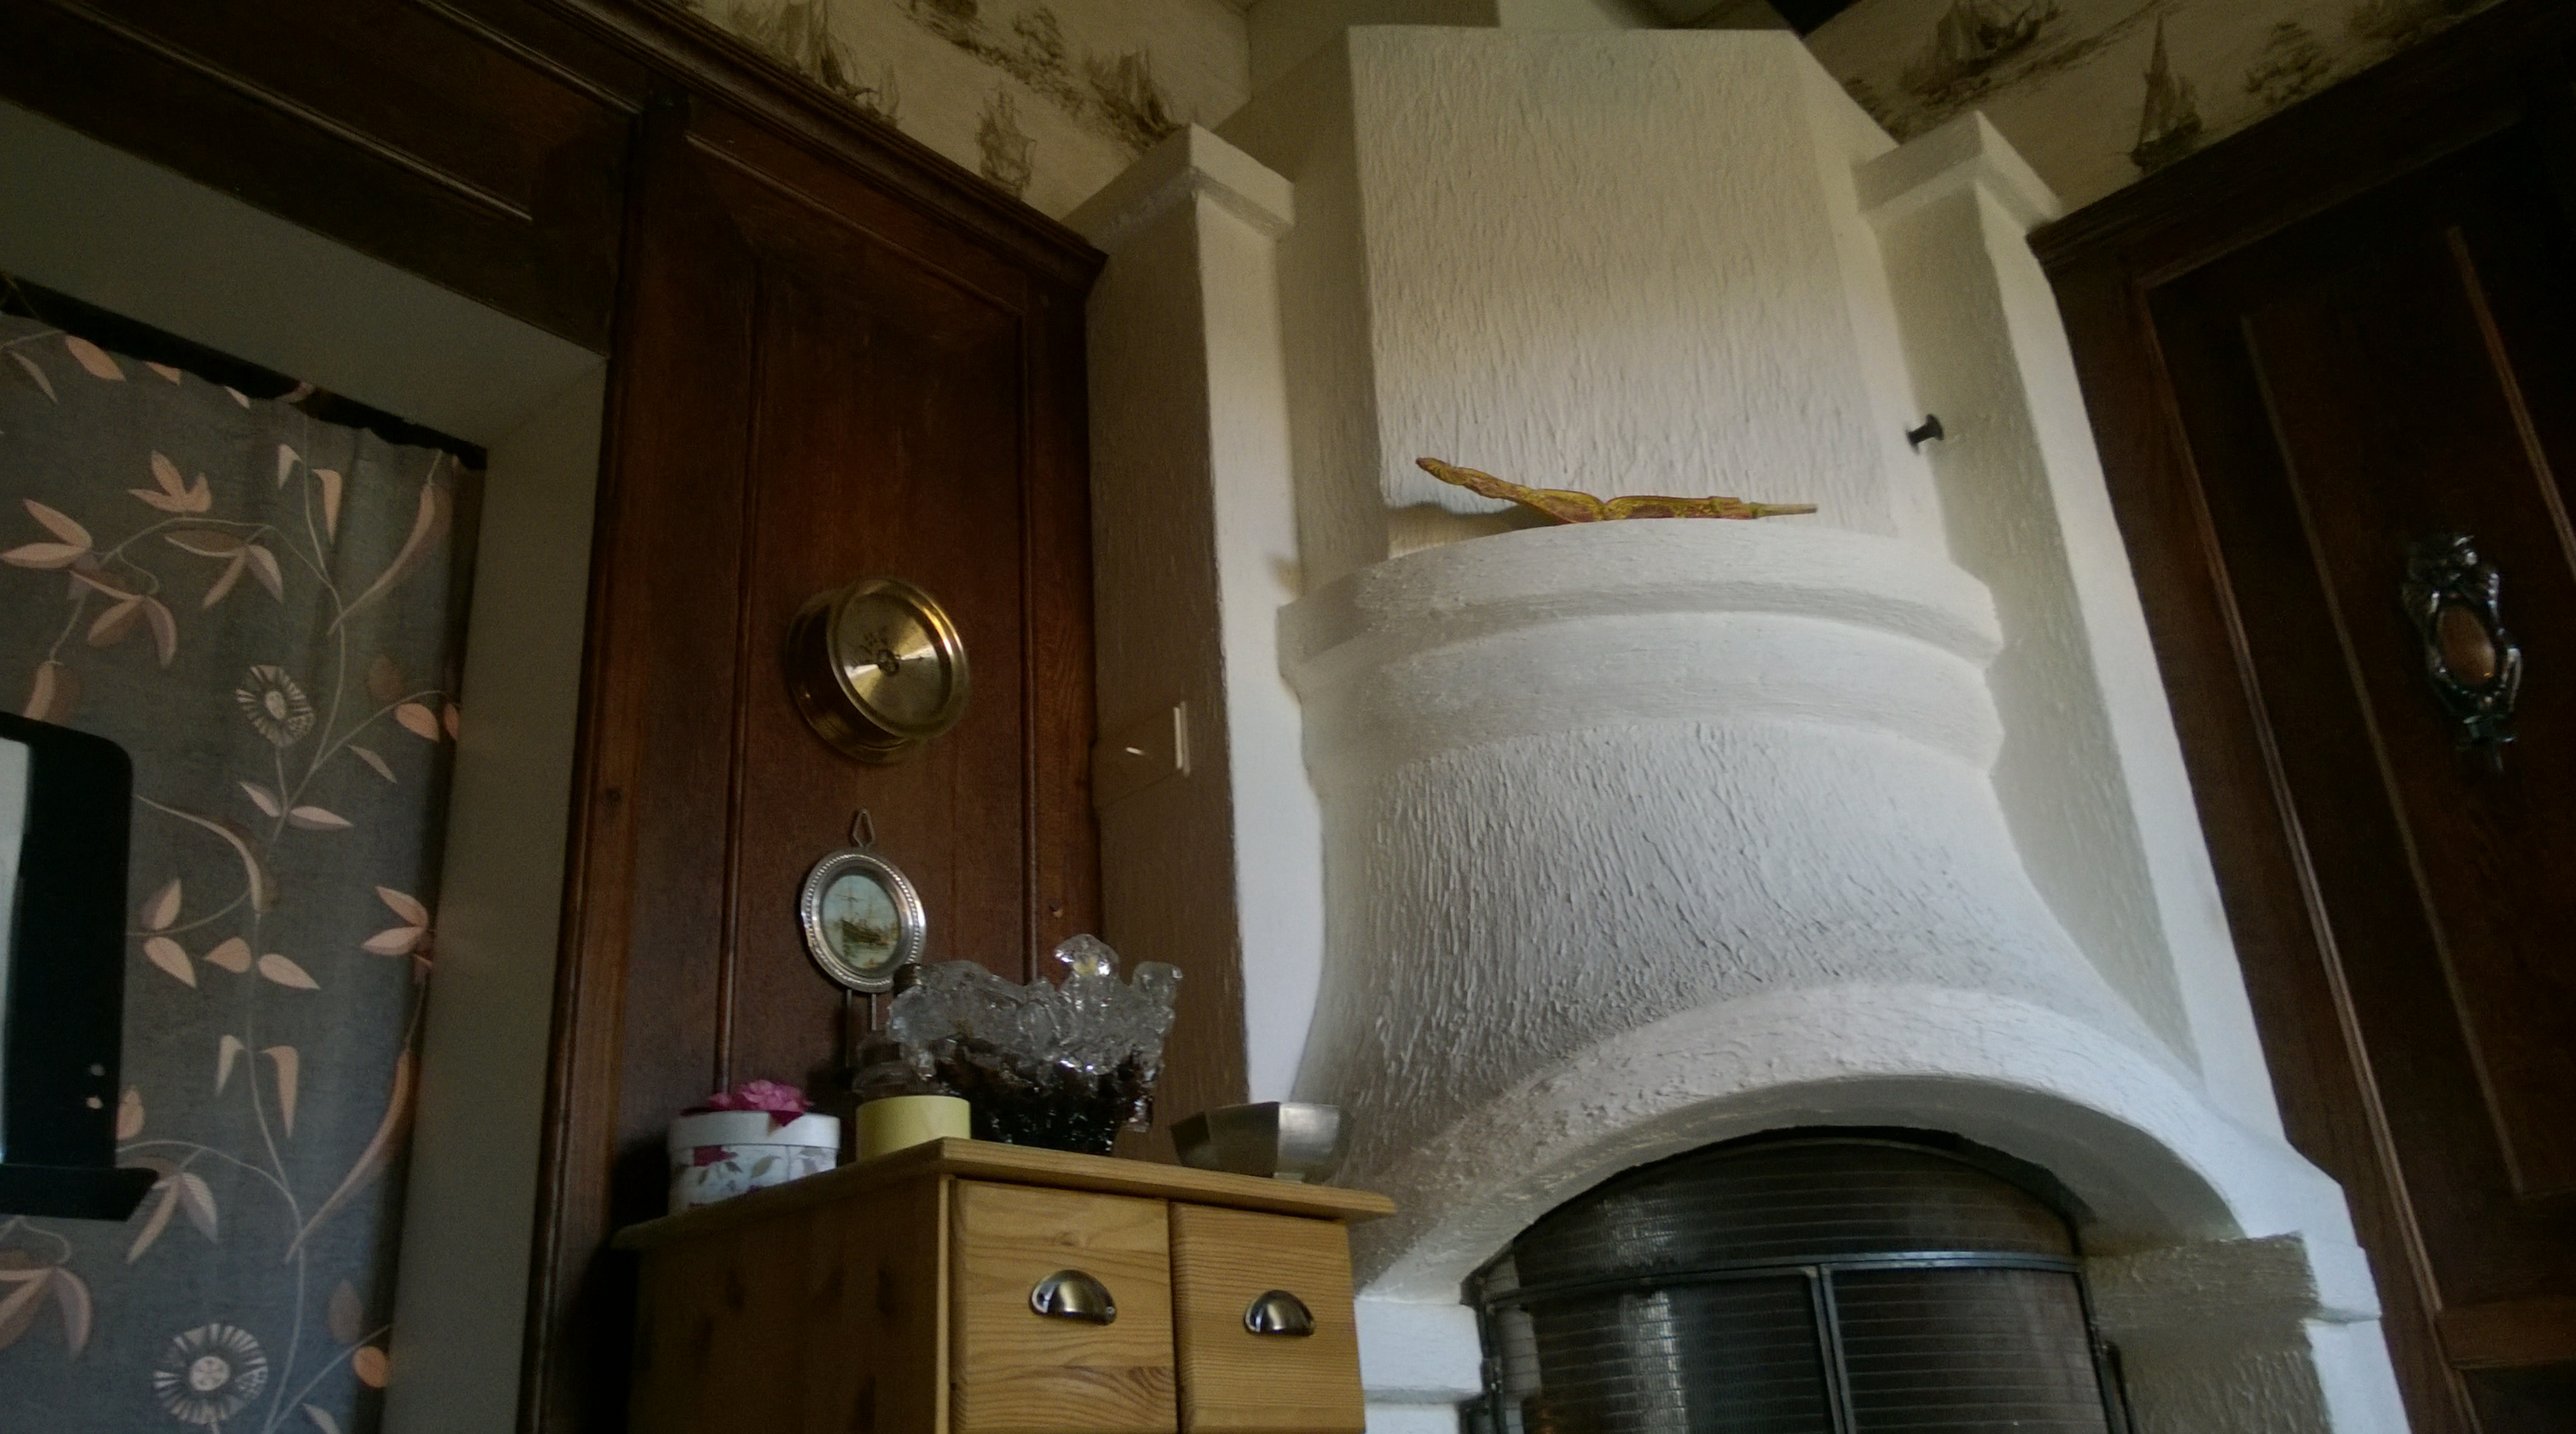
\includegraphics[width=\textwidth]{comparison_figures/library_sample.jpg}
        \caption{Library: wooden furniture and stucco fireplace}
    \end{subfigure}
    \hfill
    \begin{subfigure}{0.48\textwidth}
        \centering
        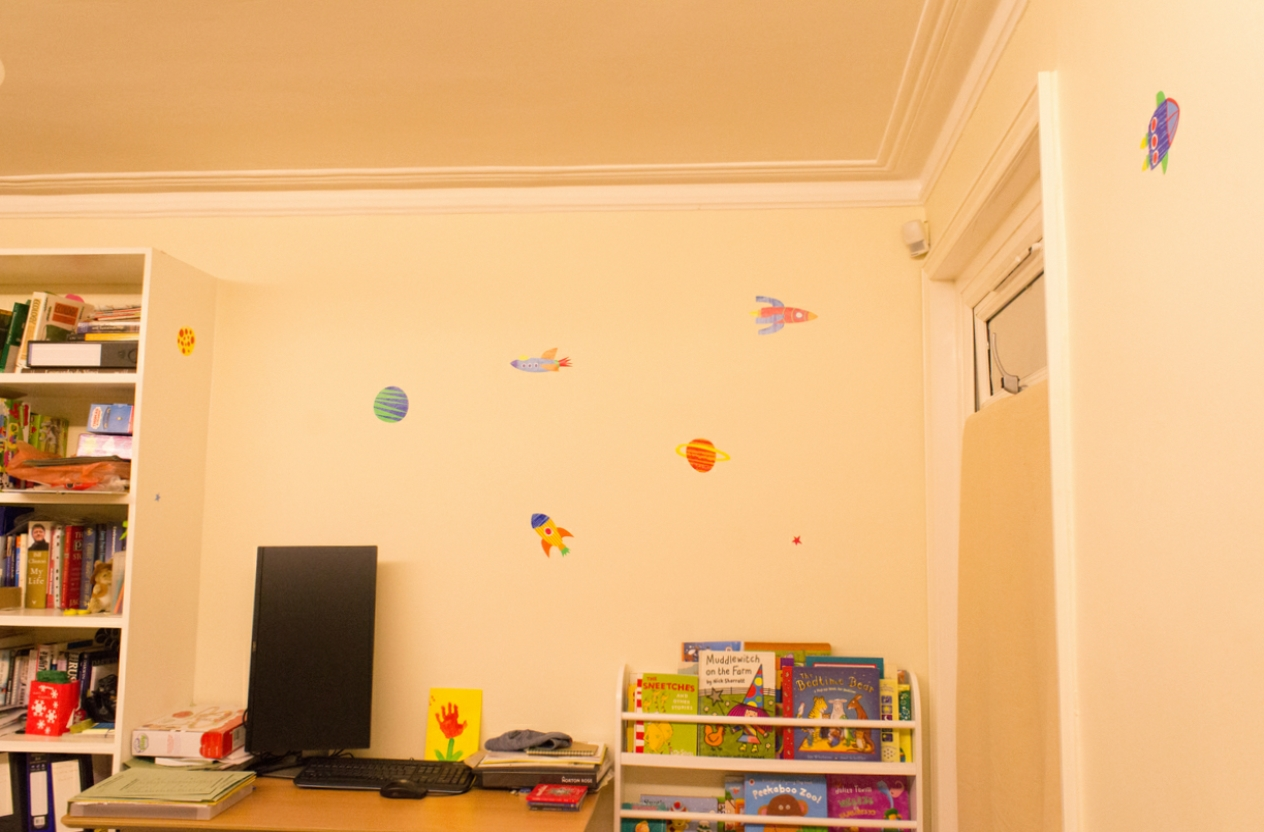
\includegraphics[width=\textwidth]{comparison_figures/playroom_sample.jpg}
        \caption{Playroom: large uniform walls and ceiling}
    \end{subfigure}
    \caption{Sample views from the three Deep Blending scenes: DrJohnson (top row), Library, and Playroom (bottom row).}
    \label{fig:dataset_samples}
\end{figure}

\section{Experimental Setup}

All experiments are conducted within a unified training framework implemented in \texttt{train.py}, which extends the PlanarGS codebase~\cite{planargs} with the geometric priors and edge-aware densification described in Chapter~4. The implementation is publicly available on GitHub.\footnote{\url{https://github.com/ArtemKrayevskiy/Geometry-regularized-Gaussian-splatting}} The optimization process runs for 30,000 iterations using the Adam optimizer~\cite{kingma2014adam}, with identical hyperparameters across all experiments. All training runs are performed on a single \textbf{NVIDIA RTX 3090} GPU (24 GB VRAM) with \textbf{CUDA 11.8} and 24 GB system RAM.

\subsection{Unified Training Pipeline}

The proposed framework is modular and controlled via command-line flags, allowing each geometric prior to be independently enabled or disabled. This design makes it possible to systematically study the contribution of each component as well as their interactions. The pipeline integrates the following components:

\begin{itemize}
    \item \textbf{Core Geometric Priors:} Depth regularization ($\mathcal{L}_{depth}$), normal consistency ($\mathcal{L}_{normal}$), planar co-planarity constraint ($\mathcal{L}_{planar}$), and scale regularization.
    \item \textbf{Edge-Aware Adaptive Control:} Spatially varying densification strategy that concentrates smaller Gaussians near structural edges while allowing larger, more efficient primitives in planar interiors.
    \item \textbf{Mesh-Based Regularization:} Optional TSDF mesh extraction used to guide geometric consistency through mesh prior constraints.
\end{itemize}

Each loss term can be disabled individually by setting its corresponding weight $\lambda$ to zero or by using explicit disable flags (e.g., \texttt{--disable\_planar}, \texttt{--disable\_depth\_prior}). This flexibility enables comprehensive ablation analysis across all possible combinations of geometric priors.

\subsection{Hyperparameters and Training Configuration}

Table~\ref{tab:hyperparameters} summarizes the key hyperparameters used across all experiments. Loss weights were chosen by manual grid search over a small validation set of held-out views from the DrJohnson scene: $\lambda_{depth} = 0.05$ was set small relative to the photometric loss to avoid over-constraining early optimization; $\lambda_{normal} = 0.2$ and $\lambda_{planar} = 0.5$ were tuned to match the magnitude of rendered normal and depth residuals, respectively; $\lambda_{scale} = 100$ acts as a strong regularizer to prevent degenerate covariance matrices. The scheduling of geometric losses follows a staged approach: depth regularization is introduced early (iteration 7,000) to stabilize optimization, while planar and normal priors are activated later (iterations 14,000 and 20,000 respectively) after initial geometry has converged.

\begin{table}[h]
\centering
\caption{Training hyperparameters and loss weights used in all experiments.}
\label{tab:hyperparameters}
\begin{tabular}{ll}
\toprule
\textbf{Parameter} & \textbf{Value} \\
\midrule
Total iterations & 30,000 \\
Optimizer & Adam \\
Learning rate (positions) & $1.6 \times 10^{-4}$ \\
Learning rate (features) & $2.5 \times 10^{-3}$ \\
\midrule
$\lambda_{dssim}$ (SSIM weight) & 0.2 \\
$\lambda_{scale}$ (scale regularization) & 100.0 \\
$\lambda_{depth}$ (depth prior) & 0.05 \\
$\lambda_{normal}$ (normal prior) & 0.2 \\
$\lambda_{planar}$ (planar constraint) & 0.5 \\
$\lambda_{edge}$ (edge normal loss) & 0.0--0.1 \\
\midrule
Depth prior start iteration & 7,000 \\
Planar loss start iteration & 14,000 \\
Normal prior start iteration & 20,000 \\
\midrule
Edge split boost factor & 2.5 \\
Center split reduction factor & 0.4 \\
Edge scale minimum ($s_{min}$) & 0.3 \\
Center scale maximum ($s_{max}$) & 2.0 \\
\midrule
TSDF voxel size & 0.02 m \\
TSDF max depth & 100.0 m \\
Mesh cleaning threshold & 1,000 triangles \\
\bottomrule
\end{tabular}
\end{table}

For edge-aware configurations, structural boundaries are detected using line segment detection (LSD)~\cite{vongioi2010lsd} on training images, and distance fields are precomputed to enable spatially adaptive densification. When mesh regularization is enabled, TSDF fusion is performed after training using Open3D~\cite{zhou2018open3d}, with rendered depth maps from all training views integrated into a volumetric representation.

\subsection{Automated Experiment Pipeline}

To ensure reproducibility and systematic evaluation, all 32 configurations are trained automatically using a batch processing script (\texttt{train\_all\_combinations.py}). For each configuration, the pipeline:

\begin{enumerate}
    \item Trains the model with \texttt{--eval} flag to enable train/test split
    \item Renders test views using \texttt{render.py}
    \item Computes metrics (PSNR, SSIM, LPIPS) using \texttt{metrics.py}
    \item Extracts statistics: training time, Gaussian count, and model file size
    \item Uploads results to a centralized repository for analysis
    \item Cleans up intermediate files to conserve disk space
\end{enumerate}

This automated workflow minimizes human error and ensures that all configurations are evaluated under identical conditions, enabling reliable comparison and reproducible research.

\section{Evaluation Metrics}
\label{sec:quality_metrics}

We evaluate reconstruction quality using three standard image-based metrics computed on held-out test views, and three efficiency metrics that capture representation compactness.

\subsection{Peak Signal-to-Noise Ratio (PSNR)}

PSNR is a pixel-wise fidelity metric derived from the Mean Squared Error (MSE) between a reconstructed image $\hat{I}$ and the ground truth $I$ of size $H \times W$:

\begin{equation}
\mathrm{MSE} = \frac{1}{HW} \sum_{i=1}^{H} \sum_{j=1}^{W} \left( I(i,j) - \hat{I}(i,j) \right)^2,
\end{equation}

\begin{equation}
\mathrm{PSNR} = 10 \cdot \log_{10} \left( \frac{L^2}{\mathrm{MSE}} \right),
\end{equation}

where $L$ is the maximum possible pixel value ($L = 255$ for 8-bit images). Higher PSNR (in dB) indicates lower pixel-wise error and better reconstruction quality.

\subsection{Structural Similarity Index Measure (SSIM)}

SSIM evaluates perceptual image quality by jointly comparing luminance, contrast, and structural information~\cite{wang2004ssim}:

\begin{equation}
\mathrm{SSIM}(I, \hat{I}) =
\frac{(2 \mu_I \mu_{\hat{I}} + C_1)(2 \sigma_{I\hat{I}} + C_2)}
{(\mu_I^2 + \mu_{\hat{I}}^2 + C_1)(\sigma_I^2 + \sigma_{\hat{I}}^2 + C_2)},
\end{equation}

where $\mu_I$, $\mu_{\hat{I}}$ are image means, $\sigma_I^2$, $\sigma_{\hat{I}}^2$ are variances, $\sigma_{I\hat{I}}$ is the covariance, and $C_1$, $C_2$ are stability constants. SSIM ranges from 0 to 1; higher values indicate greater structural similarity.

\subsection{Learned Perceptual Image Patch Similarity (LPIPS)}

LPIPS measures perceptual similarity via deep feature distances from a pretrained network~\cite{zhang2018lpips}:

\begin{equation}
\mathrm{LPIPS}(I, \hat{I}) =
\sum_{l} \frac{1}{H_l W_l}
\sum_{h,w} \left\| w_l \odot
\left( \phi_l(I)_{h,w} - \phi_l(\hat{I})_{h,w} \right) \right\|_2^2,
\end{equation}

where $\phi_l(\cdot)$ are feature maps at layer $l$, $w_l$ are learned channel-wise weights, and $\odot$ is element-wise multiplication. Lower LPIPS indicates higher perceptual similarity; it correlates better with human judgement than PSNR~\cite{kerbl20233dgs}.

\subsection{Efficiency Metrics}

In addition to visual quality, we report three representation efficiency metrics:

\begin{itemize}
    \item \textbf{Number of Gaussians ($|\mathcal{G}|$):} The total primitive count in the final model, defined as:
    \begin{equation}
        |\mathcal{G}| = \sum_{k=1}^{K} \mathbf{1}[\alpha_k > \alpha_{\min}],
    \end{equation}
    where $\alpha_k$ is the opacity of the $k$-th Gaussian and $\alpha_{\min}$ is a pruning threshold. This count is extracted directly from the PLY file header and reflects model compactness.

    \item \textbf{Model Size:} File size of the stored point cloud in megabytes (MB), which directly determines storage and transmission costs.

    \item \textbf{Training Time:} Wall-clock time in minutes to complete 30,000 training iterations, measuring computational overhead introduced by each prior.
\end{itemize}

These efficiency metrics are important when the final model must be stored, transmitted, or rendered on hardware with limited memory.

\section{Research Hypotheses}

The experiments are designed to test five hypotheses derived from the research gap identified in Chapter~2:

\begin{enumerate}
    \item \textbf{Complementarity of Geometric Priors:} Combining depth, normals, and planarity should improve reconstruction quality beyond what any single prior achieves, since each modality constrains a different aspect of scene geometry.

    \item \textbf{Redundancy Under Stronger Supervision:} A related question is whether certain priors become superfluous when a stronger cue is already active — for instance, whether normal consistency adds value once both depth and planarity constraints are in place.

    \item \textbf{Structural Priors Dominate in Planar Scenes:} In indoor environments where walls, floors, and ceilings account for most of the visible surface area, edge and planarity constraints are expected to matter more than per-pixel normal cues, which capture only local surface orientation.

    \item \textbf{Compactness Through Geometry:} Geometric priors that discourage unnecessary densification on flat surfaces should yield smaller models without sacrificing rendering quality, reducing the total primitive count below that of the photometric-only baseline.

    \item \textbf{Edge-Aware Densification Improves Efficiency:} Concentrating smaller primitives near structural boundaries while allowing larger ones to grow in flat interiors should simultaneously improve sharpness at edges and reduce the overall Gaussian count.
\end{enumerate}

All five hypotheses are tested by comparing the 32 geometric prior combinations against the baseline in Table~A.1 (Appendix~\ref{appendix:ablation}).

\section{Ablation Study}

To analyze the contribution of different geometric priors, we perform a comprehensive ablation study over all combinations of five binary modalities:

\begin{itemize}
    \item \textbf{N (Normals):} Normal prior loss ($\mathcal{L}_{normal}$) that aligns rendered normals with monocular normal estimates.
    \item \textbf{D (Depth):} Depth prior loss ($\mathcal{L}_{depth}$) that enforces consistency with monocular depth predictions.
    \item \textbf{P (Planarity):} Planar co-planarity constraint ($\mathcal{L}_{planar}$) that encourages Gaussians within segmented planar regions to lie on a common plane.
    \item \textbf{M (Mesh):} Mesh-based regularization through TSDF fusion, which provides additional geometric supervision and enables mesh extraction.
    \item \textbf{E (Edges):} Edge-aware adaptive densification that concentrates smaller Gaussians near structural boundaries while using larger primitives in planar interiors.
\end{itemize}

This results in $2^5 = 32$ unique configurations, ranging from the \textit{baseline} (all priors disabled) to the \textit{full} configuration (all priors enabled). Each configuration is trained independently for 30,000 iterations using identical hyperparameters. All runs use a single fixed random seed; variance across seeds is not quantified, so the reported differences should be interpreted with appropriate caution given the small absolute magnitudes involved.

The systematic exploration of this configuration space allows us to identify which priors contribute most to reconstruction quality and efficiency and to detect redundancies or negative interactions. All 32 configurations with their prior combinations are listed in Table~A.1 (Appendix~\ref{appendix:ablation}), and the full quantitative results for all 33 configurations (32 ablation + \textit{original} row) are in Table~A.2 (Appendix~\ref{appendix:ablation}).

\section{Results and Discussion}

The experimental results reveal several consistent patterns in the interplay between different geometric regularization strategies.

\subsection{Overall Performance Trends}

Tables~\ref{tab:summary_drjohnson}--\ref{tab:summary_playroom} show key configurations for each of the three scenes individually. The \textit{original} row refers to unmodified PlanarGS with default settings; \textit{baseline} is our framework with all five priors disabled. The small PSNR difference between original and baseline (e.g., 29.08 vs.\ 29.03 dB on DrJohnson) reflects minor implementation differences between the PlanarGS codebase and our modified training pipeline. Full results for all 33 configurations are in Appendix~\ref{appendix:ablation}.

% ---- Table 5.2: DrJohnson per-scene summary ----
\begin{table}[t]
\centering\small
\caption{Key configurations --- DrJohnson scene. Full per-scene results in Appendix~\ref{appendix:ablation}.}
\label{tab:summary_drjohnson}
\begin{tabular}{@{}l|ccc|ccc@{}}
\toprule
\textbf{Configuration} & \textbf{PSNR~↑} & \textbf{SSIM~↑} & \textbf{LPIPS~↓} & \textbf{Gs.(K)~↓} & \textbf{Size(MB)~↓} & \textbf{Time(min)} \\
\midrule
original (PlanarGS) & 29.08 & 0.902 & 0.252 & 1690 & 400 & 44.6 \\
\midrule
baseline (no priors) & 29.03 & 0.903 & 0.252 & 1704 & 403 & 44.0 \\
depths & \textbf{29.16} & 0.903 & 0.250 & 1703 & 403 & 44.1 \\
normals & 29.06 & 0.902 & 0.252 & 1696 & 401 & 44.1 \\
planarity & 29.06 & 0.903 & 0.250 & 1693 & 400 & 44.2 \\
meshes & 29.11 & \textbf{0.904} & \textbf{0.249} & 1707 & 404 & 122.8 \\
\midrule
edges & 28.70 & 0.898 & 0.269 & 988 & 234 & 43.2 \\
\midrule
depths\_planarity & 29.08 & 0.903 & 0.252 & 1698 & 402 & 44.6 \\
meshes\_edges & 28.67 & 0.897 & 0.273 & \textbf{964} & \textbf{228} & 83.6 \\
normals\_depths\_edges & 27.71 & 0.889 & 0.280 & 979 & 232 & 44.5 \\
\midrule
all priors (full) & 28.69 & 0.898 & 0.269 & 989 & 234 & 89.2 \\
\bottomrule
\end{tabular}
\end{table}

% ---- Table 5.3: Library per-scene summary ----
\begin{table}[t]
\centering\small
\caption{Key configurations --- Library scene. Full per-scene results in Appendix~\ref{appendix:ablation}.}
\label{tab:summary_library}
\begin{tabular}{@{}l|ccc|ccc@{}}
\toprule
\textbf{Configuration} & \textbf{PSNR~↑} & \textbf{SSIM~↑} & \textbf{LPIPS~↓} & \textbf{Gs.(K)~↓} & \textbf{Size(MB)~↓} & \textbf{Time(min)} \\
\midrule
original (PlanarGS) & 24.10 & 0.782 & \textbf{0.366} & 1757 & 416 & 47.7 \\
\midrule
baseline (no priors) & \textbf{24.13} & 0.782 & 0.366 & 1761 & 417 & 48.8 \\
depths & 24.12 & 0.781 & 0.366 & 1782 & 422 & 47.7 \\
normals & 24.10 & 0.782 & 0.366 & 1776 & 420 & 48.0 \\
planarity & 24.06 & 0.782 & 0.366 & 1784 & 422 & 49.1 \\
meshes & 24.11 & 0.782 & 0.366 & 1775 & 420 & 326.0 \\
\midrule
edges & 24.07 & \textbf{0.785} & 0.372 & 1239 & 293 & 49.2 \\
\midrule
depths\_planarity & \textbf{24.13} & 0.782 & 0.366 & 1788 & 423 & 48.8 \\
meshes\_edges & 23.92 & 0.783 & 0.375 & 1227 & 290 & 206.8 \\
normals\_depths\_edges & 23.97 & 0.784 & 0.376 & \textbf{1221} & \textbf{289} & 48.0 \\
\midrule
all priors (full) & 23.98 & 0.783 & 0.374 & 1231 & 291 & 206.2 \\
\bottomrule
\end{tabular}
\end{table}

% ---- Table 5.4: Playroom per-scene summary ----
\begin{table}[t]
\centering\small
\caption{Key configurations --- Playroom scene. Full per-scene results in Appendix~\ref{appendix:ablation}.}
\label{tab:summary_playroom}
\begin{tabular}{@{}l|ccc|ccc@{}}
\toprule
\textbf{Configuration} & \textbf{PSNR~↑} & \textbf{SSIM~↑} & \textbf{LPIPS~↓} & \textbf{Gs.(K)~↓} & \textbf{Size(MB)~↓} & \textbf{Time(min)} \\
\midrule
original (PlanarGS) & 30.37 & 0.910 & 0.250 & 1202 & 285 & 39.3 \\
\midrule
baseline (no priors) & 30.48 & 0.910 & 0.249 & 1214 & 287 & 39.6 \\
depths & 30.35 & 0.909 & 0.249 & 1217 & 288 & 38.6 \\
normals & 30.43 & 0.909 & 0.249 & 1209 & 286 & 39.8 \\
planarity & 30.42 & 0.910 & 0.249 & 1213 & 287 & 38.3 \\
meshes & 30.46 & 0.910 & 0.249 & 1217 & 288 & 70.2 \\
\midrule
edges & 30.14 & 0.907 & 0.255 & \textbf{956} & \textbf{226} & 39.7 \\
\midrule
depths\_planarity & \textbf{30.54} & \textbf{0.911} & \textbf{0.248} & 1223 & 289 & 39.9 \\
meshes\_edges & 30.16 & 0.908 & 0.253 & 969 & 229 & 67.5 \\
normals\_depths\_edges & 30.14 & 0.909 & 0.254 & 958 & 227 & 40.0 \\
\midrule
all priors (full) & 30.23 & 0.908 & 0.255 & 957 & 226 & 66.6 \\
\bottomrule
\end{tabular}
\end{table}

Across all three scenes the results show a consistent pattern: individual priors have minimal standalone PSNR impact, combinations matter, and edge-aware densification is the only prior with a large compactness effect. The top-performing configurations per scene are:
\begin{itemize}
    \item \textbf{Best PSNR:} \textit{depths\_planarity} across all three scenes (29.08 / 24.13 / 30.54 dB for DrJohnson / Library / Playroom).
    \item \textbf{Most Compact:} edge-containing configs reduce Gaussian count by 30--35\% on each scene (e.g., \textit{meshes\_edges}: 964K / 1{,}227K / 969K Gaussians).
    \item \textbf{Most Expensive:} mesh-based priors add $3$--$7\times$ training overhead (e.g., 326 min vs.\ 49 min on Library).
\end{itemize}

Simpler configurations often outperform the full configuration — certain prior combinations introduce conflicting gradients that hurt optimization.

Returning to the five research hypotheses stated in Section~5.4: \textbf{H1} (complementarity) is \textit{partially supported} — depths\_planarity achieves +0.04 dB above baseline, but most individual priors do not improve PSNR individually. \textbf{H2} (redundancy under stronger supervision) is \textit{supported} — normal priors add little once depth and planarity are active. \textbf{H3} (structural priors dominate in planar scenes) is \textit{partially supported} — planarity improves quality in combinations, but edge-aware densification has the largest single-prior effect on compactness. \textbf{H4} (compactness through geometry) is \textit{supported} — edge-aware configurations reduce Gaussian count by 30--32\% with only a modest quality trade-off. \textbf{H5} (edge-aware densification improves efficiency) is \textit{supported} — edge-aware is the only prior that substantially reduces model size across all combinations that include it.

\subsection{Individual Prior Contributions}

Isolating each modality reveals that most geometric priors have minimal standalone impact on PSNR but affect compactness and training cost in different ways.

Table~\ref{tab:individual_priors} summarizes the standalone effect of each prior.

\begin{table}[h]
\centering
\small
\caption{Individual prior contributions vs.\ baseline (27.88 dB, 1560K Gaussians, 369~MB). $\Delta$PSNR and $\Delta$Gs.\ are differences from baseline.}
\label{tab:individual_priors}
\begin{tabular}{l|cccc|cc}
\toprule
\textbf{Prior} & \textbf{PSNR} & \textbf{$\Delta$PSNR} & \textbf{Gs.(K)} & \textbf{$\Delta$Gs.} & \textbf{Size(MB)} & \textbf{Time(min)} \\
\midrule
Depth (D)     & 27.88 & 0.00  & 1568 & +8   & 371 & 43.5 \\
Normals (N)   & 27.86 & $-$0.02 & 1561 & +1   & 369 & 44.0 \\
Planarity (P) & 27.85 & $-$0.03 & 1564 & +4   & 370 & 43.9 \\
Mesh (M)      & 27.89 & +0.01 & 1567 & +7   & 371 & 173.0 \\
Edges (E)     & 27.64 & $-$0.24 & 1061 & $-$499 & 251 & 44.0 \\
\bottomrule
\end{tabular}
\end{table}

The depth prior (27.88 dB) is identical to the baseline in isolation, stabilizing optimization in textureless regions without changing the overall Gaussian count. Normal supervision (27.86 dB) and planarity (27.85 dB) each show a negligible difference of at most $-0.03$ dB from the baseline. Mesh-based regularization is the only single prior with a measurable positive PSNR effect (+0.01 dB, 27.89 dB), but it adds no compactness benefit and increases training time by roughly $4\times$ due to TSDF fusion overhead.

The key insight is that priors become meaningful in \emph{combinations}. The pair depths\_planarity achieves the best rendering quality at 27.92 dB (+0.04 dB above baseline), confirming complementarity between monocular depth supervision and structural planarity constraints. This modest but consistent improvement is reproducible across several two- and three-prior combinations that include both depth and planarity.

Edge-aware adaptive densification stands apart as the only modality with a large effect on model compactness: it reduces the average Gaussian count by 30--32\% (from $\sim$1{,}560K to $\sim$1{,}060K, 369 MB to $\sim$250 MB) at a PSNR cost of 0.24 dB when used alone (27.64 dB vs.\ baseline 27.88 dB). This trade-off is the primary mechanism for model size reduction and is the most practically valuable contribution when storage or memory are constrained.

\subsection{Best Performing Configurations}

The full results table (Appendix~\ref{appendix:ablation}, Table~A.2) reveals several consistent trade-offs between quality, compactness, and training cost across the 33 configurations.

The highest PSNR is achieved by \textit{depths\_planarity} (27.92 dB), confirming that combining monocular depth supervision with structural planarity constraints provides effective geometric guidance without over-constraining optimization. This two-prior combination outperforms the baseline (27.88 dB) despite using a comparable number of Gaussians (1,570K vs.\ 1,560K). \textit{normals\_meshes} and \textit{planarity\_meshes} both reach 27.90 dB, showing that even a single well-chosen prior can match or slightly exceed baseline quality.

The most compact representations consistently come from configurations that include edge-aware control. \textit{normals\_depths\_edges} requires only 1,053K Gaussians — a 32\% reduction from the baseline — while achieving 27.27 dB PSNR, 0.861 SSIM, and 0.304 LPIPS. \textit{meshes\_edges} reaches 27.58 dB PSNR, 0.863 SSIM, and 0.300 LPIPS at 1,054K Gaussians. In both cases the quality drop is small enough to be imperceptible under normal viewing conditions.

Adding planarity constraints reliably improves quality across prior combinations. The pair \textit{depths} (27.88 dB) vs.\ \textit{depths\_planarity} (27.92 dB) illustrates a consistent +0.04 dB gain from planarity alone; \textit{normals\_depths} and \textit{normals\_depths\_planarity} show a similar pattern. Beyond quality, planarity reduces over-densification on flat surfaces, keeping Gaussian count from growing unnecessarily.

The computational cost of mesh-based regularization is substantial. Training time rises from approximately 44 minutes to 174--183 minutes (nearly 4$\times$ longer) due to TSDF fusion and mesh cleaning. A direct comparison makes this concrete: \textit{depths\_meshes} achieves 27.85 dB in 182.9 minutes, while \textit{depths\_planarity} achieves better quality (27.92 dB) in 44.4 minutes. Mesh priors are therefore only justified when an explicit surface mesh is needed for downstream processing — they provide little benefit for rendering quality alone.

The full configuration with all five priors enabled achieves only 27.63 dB, well below simpler combinations such as \textit{depths\_planarity} (27.92 dB). This indicates that certain prior combinations introduce competing gradients that impede convergence; adding constraints without considering their interactions can hurt rather than help. The full configuration is compact (1,059K Gaussians), but the quality penalty is measurable and avoidable.

For maximum rendering quality, \textit{depths\_planarity} (27.92 dB PSNR, 0.865 SSIM, 0.288 LPIPS) is the recommended configuration. When model size is the primary constraint, \textit{normals\_depths\_edges} (27.27 dB PSNR, 0.861 SSIM, 0.304 LPIPS, 1{,}053K Gaussians) reduces the primitive count by 32\% with a quality gap that remains imperceptible in most viewing conditions.

\subsection{Efficiency Analysis}

The trade-off between rendering quality and Gaussian count across all 33 configurations reveals a consistent pattern.

Configurations with edge-aware control consistently require 30--32\% fewer Gaussians than their non-edge counterparts at comparable PSNR levels. The baseline reaches 27.88 dB at 1,560K Gaussians; adding edge-aware control to a depth-planarity configuration (\textit{depths\_planarity\_edges}) gives 27.61 dB at 1,065K Gaussians. Accepting a 0.3--0.6 dB PSNR reduction therefore yields a roughly one-third reduction in model size, driven by the spatially adaptive densification strategy that concentrates primitives near structural boundaries and suppresses growth in flat interiors.

Training time varies more strongly with mesh regularization than with any other prior. Edge-aware densification adds only 2--3\% overhead compared to an equivalent non-edge run. Mesh-based priors, by contrast, require TSDF fusion and mesh cleaning after training, raising total time from approximately 44 minutes to 174--175 minutes — a 4$\times$ increase. For configurations without explicit mesh extraction requirements, this overhead is difficult to justify given the modest quality gains.

Model file sizes scale directly with Gaussian count, so the 30\% reduction in primitives achieved by edge-aware configurations translates to a proportional reduction in storage without any additional compression.

\subsection{Comparison with Baseline Methods}

Table~\ref{tab:method_comparison} presents a quantitative comparison of our method against three baselines on the DrJohnson scene. DrJohnson is selected for this comparison because it is the only scene for which we have fully evaluated all competitor methods under controlled conditions at 30{,}000 training iterations. Averaged across three scenes, the ablation baseline achieves 27.88 dB PSNR (see Appendix~\ref{appendix:ablation}, Table~A.2); the DrJohnson-only numbers (Table~\ref{tab:method_comparison}) are higher (28.67 dB for Ours) because DrJohnson is a relatively easier indoor scene.

\begin{table}[h]
\centering
\caption{Quantitative comparison on the DrJohnson scene at 30{,}000 training iterations. All PLY model sizes measured on the same hardware.}
\label{tab:method_comparison}
\begin{tabular}{lcccc}
\toprule
\textbf{Method} & \textbf{PSNR~↑} & \textbf{SSIM~↑} & \textbf{LPIPS~↓} & \textbf{Size~↓} \\
\midrule
3D Gaussian Splatting~\cite{kerbl20233dgs} & 29.31 & 0.902 & 0.240 & 740 MB \\
GeoGaussian~\cite{geogaussian}             & 28.65 & 0.894 & 0.130 & 281 MB \\
PlanarGS~\cite{planargs}                   & 28.98 & 0.904 & 0.250 & 410 MB \\
Ours (depths\_planarity\_edges)            & 28.67 & 0.898 & 0.269 & \textbf{222 MB} \\
\bottomrule
\end{tabular}
\end{table}

Our method matches GeoGaussian's PSNR while achieving a 21\% smaller model (222~MB vs.\ 281~MB), and is 46\% smaller than PlanarGS (222~MB vs.\ 410~MB) with a 0.31 dB PSNR difference — a trade-off that is primarily driven by edge-aware densification. GeoGaussian achieves a notably lower LPIPS (0.130) because its dense depth/normal initialization produces perceptually sharper renders, a direction orthogonal to our compactness focus.

\subsection{Qualitative Comparison: Compactness vs.~Rendering Quality}

Beyond quantitative metrics, we present qualitative visual comparisons demonstrating that our method achieves significant model size reduction while preserving rendering quality. Figure~\ref{fig:qualitative_comparison} shows renders from the DrJohnson scene across five rows (ground truth, 3D-GS, GeoGaussian, PlanarGS, and our method) at four viewpoints. The fourth view (hallway scene) highlights a case where GeoGaussian introduces floating artifacts in the ceiling — visible in the red-boxed region — that are absent in the other methods.

\begin{figure}[p]
    \centering
    \setlength{\tabcolsep}{2pt}
    \renewcommand{\arraystretch}{0.5}
    \begin{tabular}{cccc}
        \small View 1 & \small View 2 & \small View 3 & \small View 4 \\[2pt]
        % Ground Truth row
        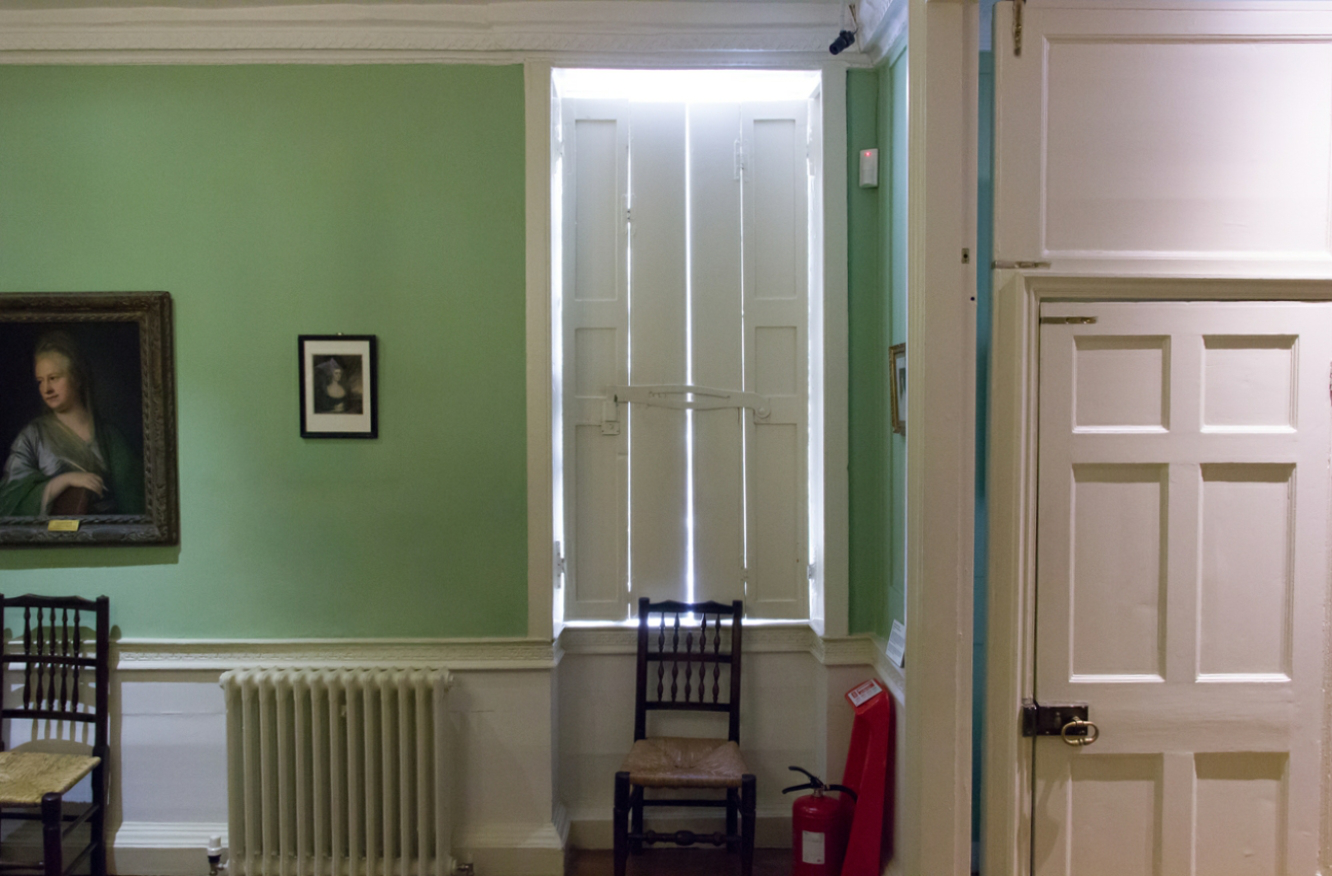
\includegraphics[width=0.235\textwidth]{comparison_figures/drjohnson_gt_view01.png} &
        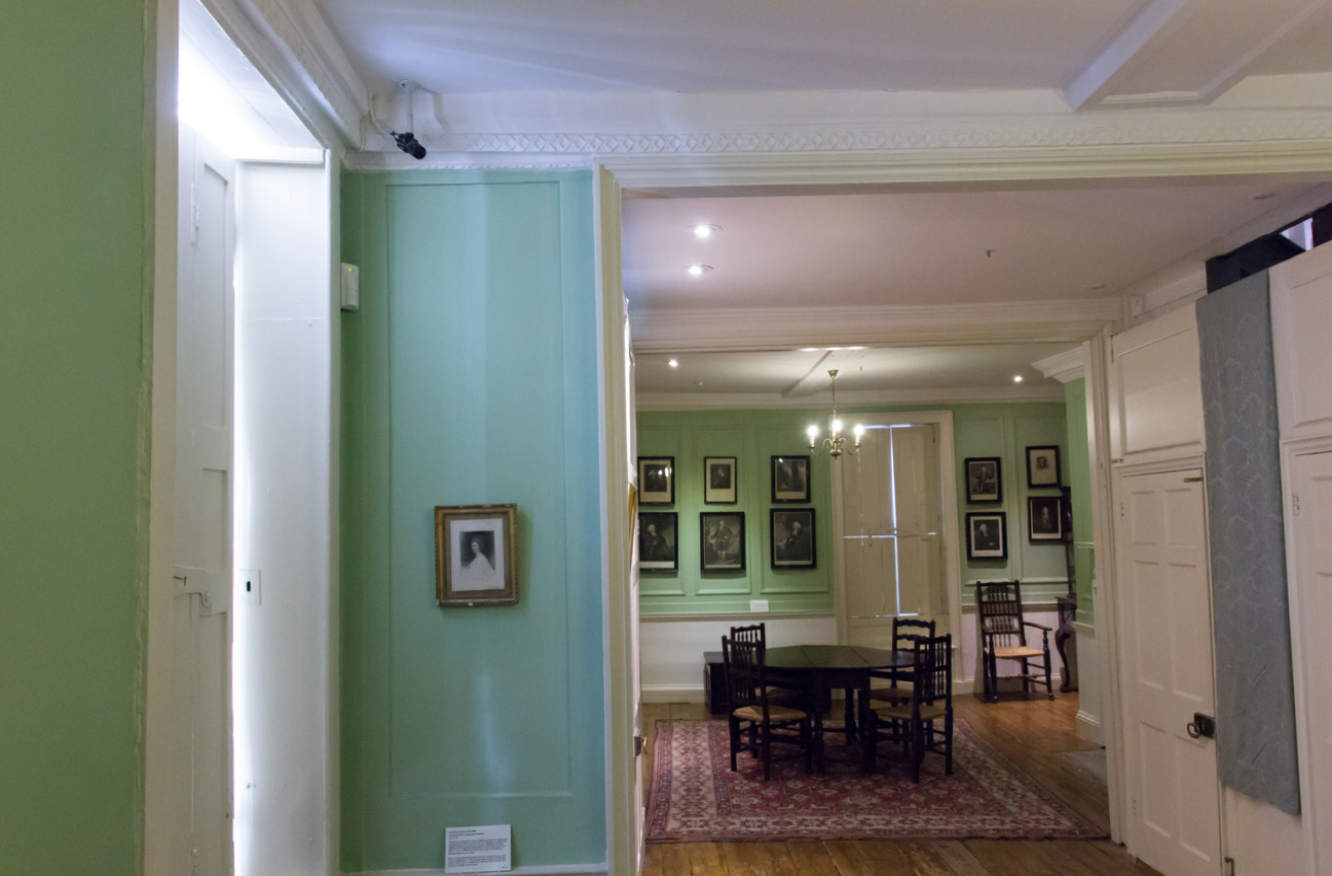
\includegraphics[width=0.235\textwidth]{comparison_figures/drjohnson_gt_view03.png} &
        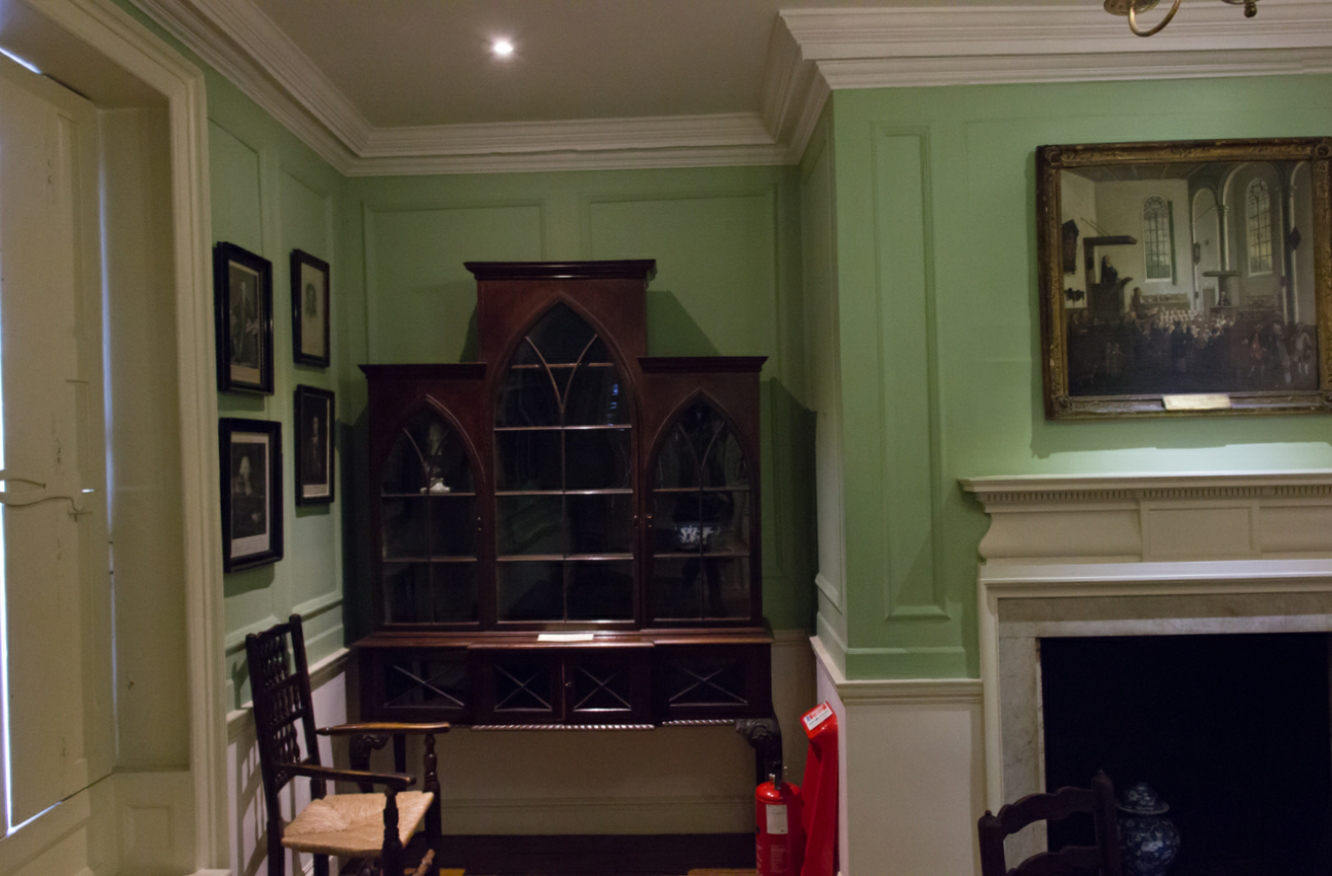
\includegraphics[width=0.235\textwidth]{comparison_figures/drjohnson_gt_view04.png} &
        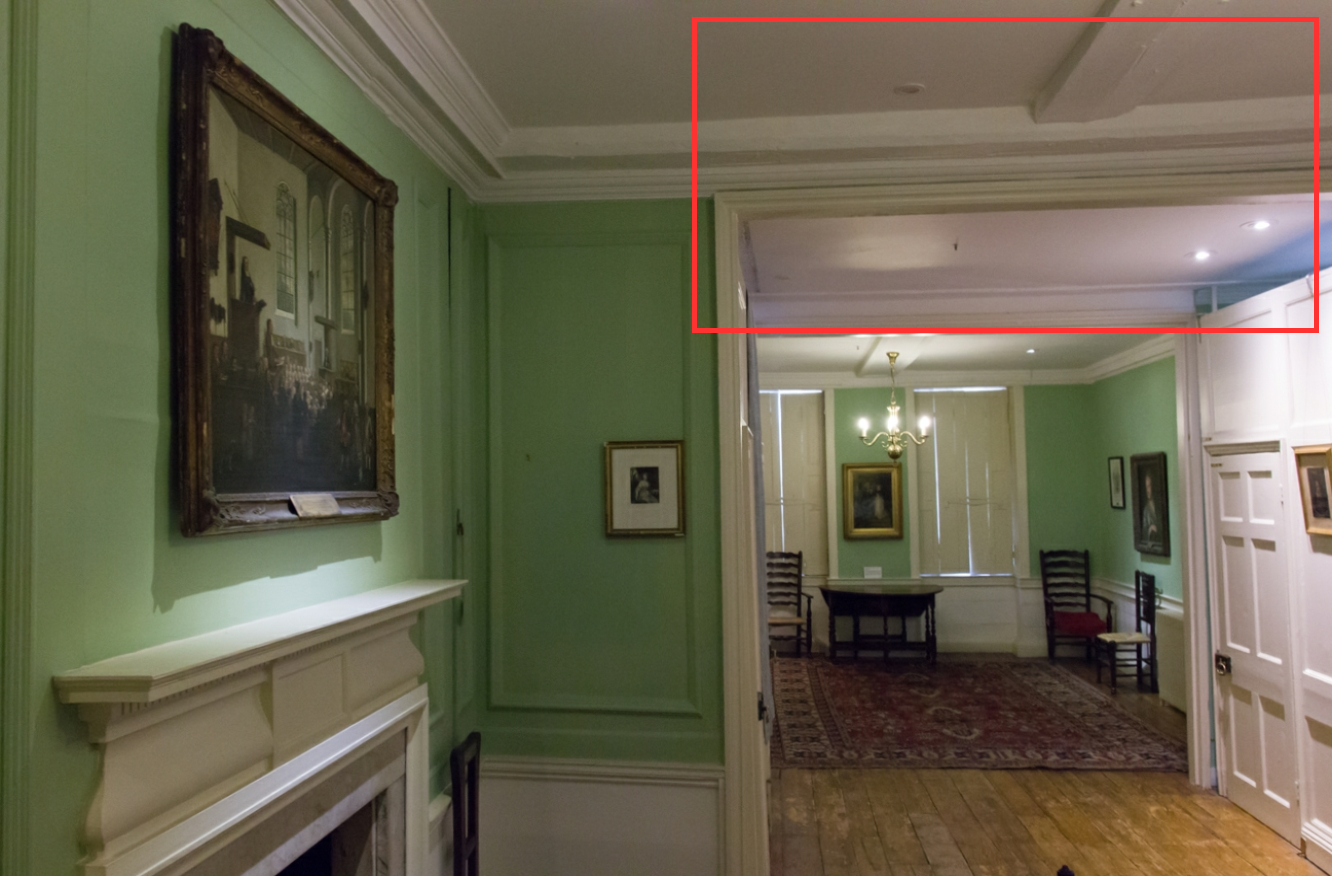
\includegraphics[width=0.235\textwidth]{comparison_figures/drjohnson_gt_view06_rect.png} \\
        \multicolumn{4}{c}{\small\textbf{(a) Ground Truth}} \\[4pt]
        % 3D-GS row
        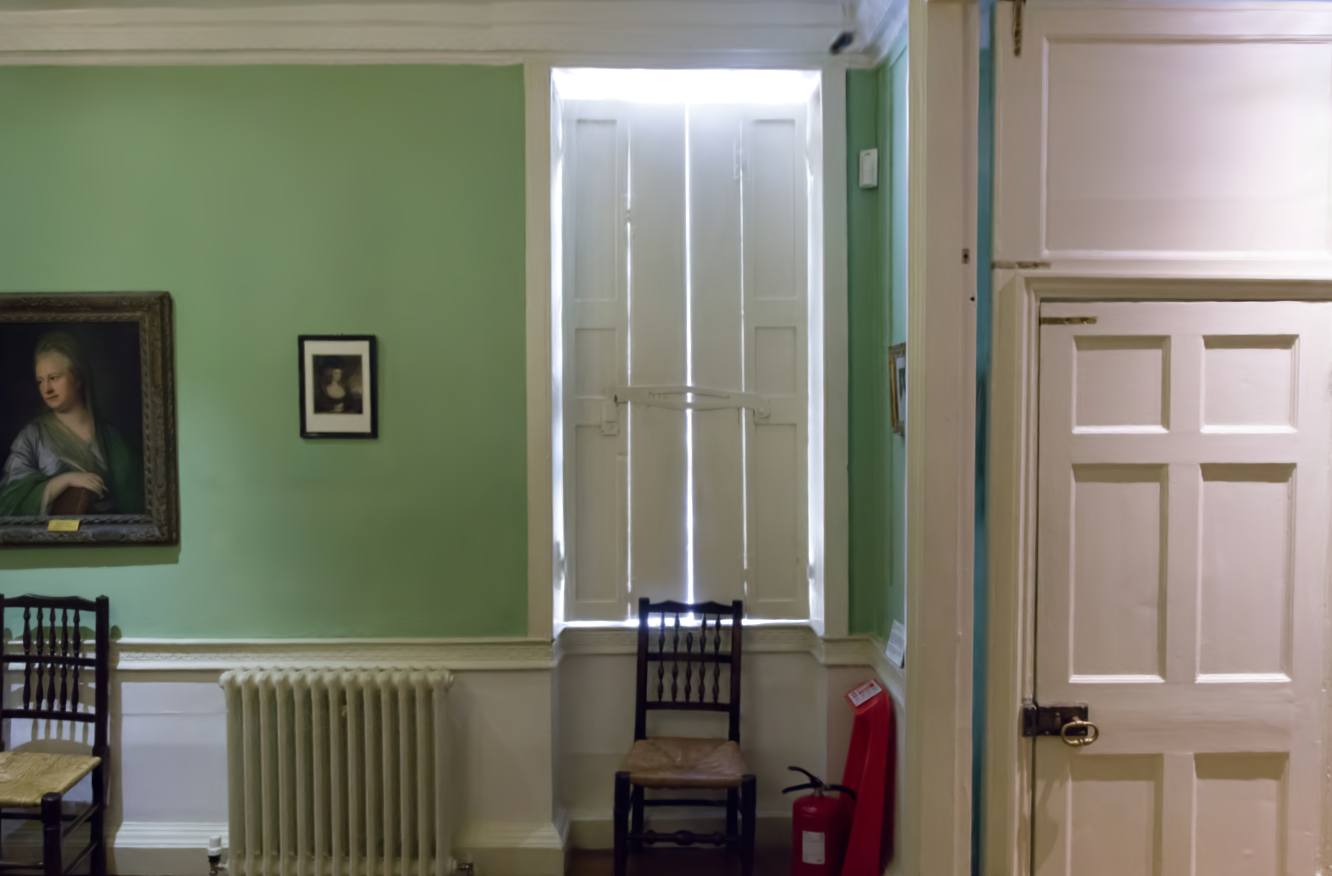
\includegraphics[width=0.235\textwidth]{comparison_figures/view_01_3DGS_original.png} &
        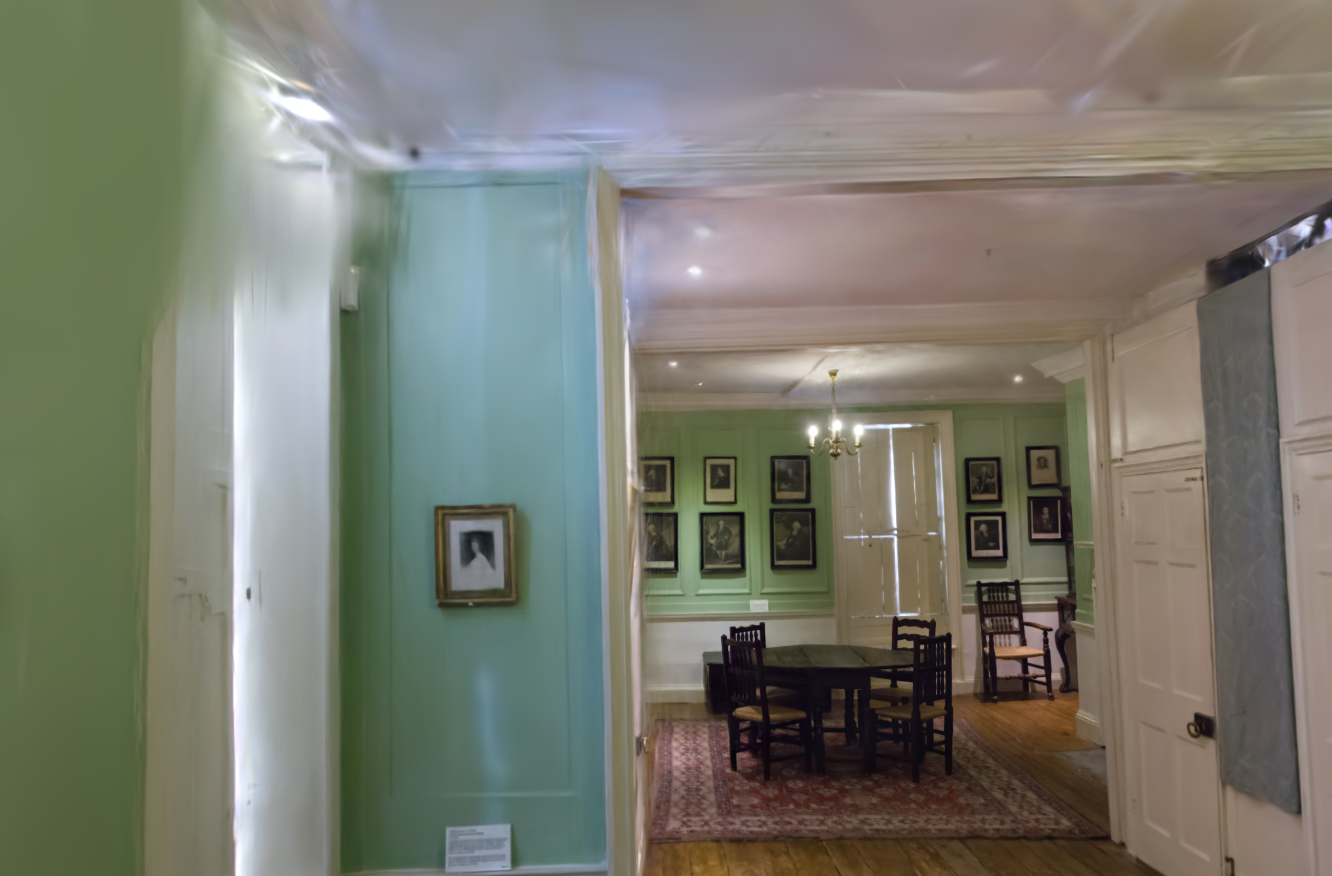
\includegraphics[width=0.235\textwidth]{comparison_figures/view_03_3DGS_Original.png} &
        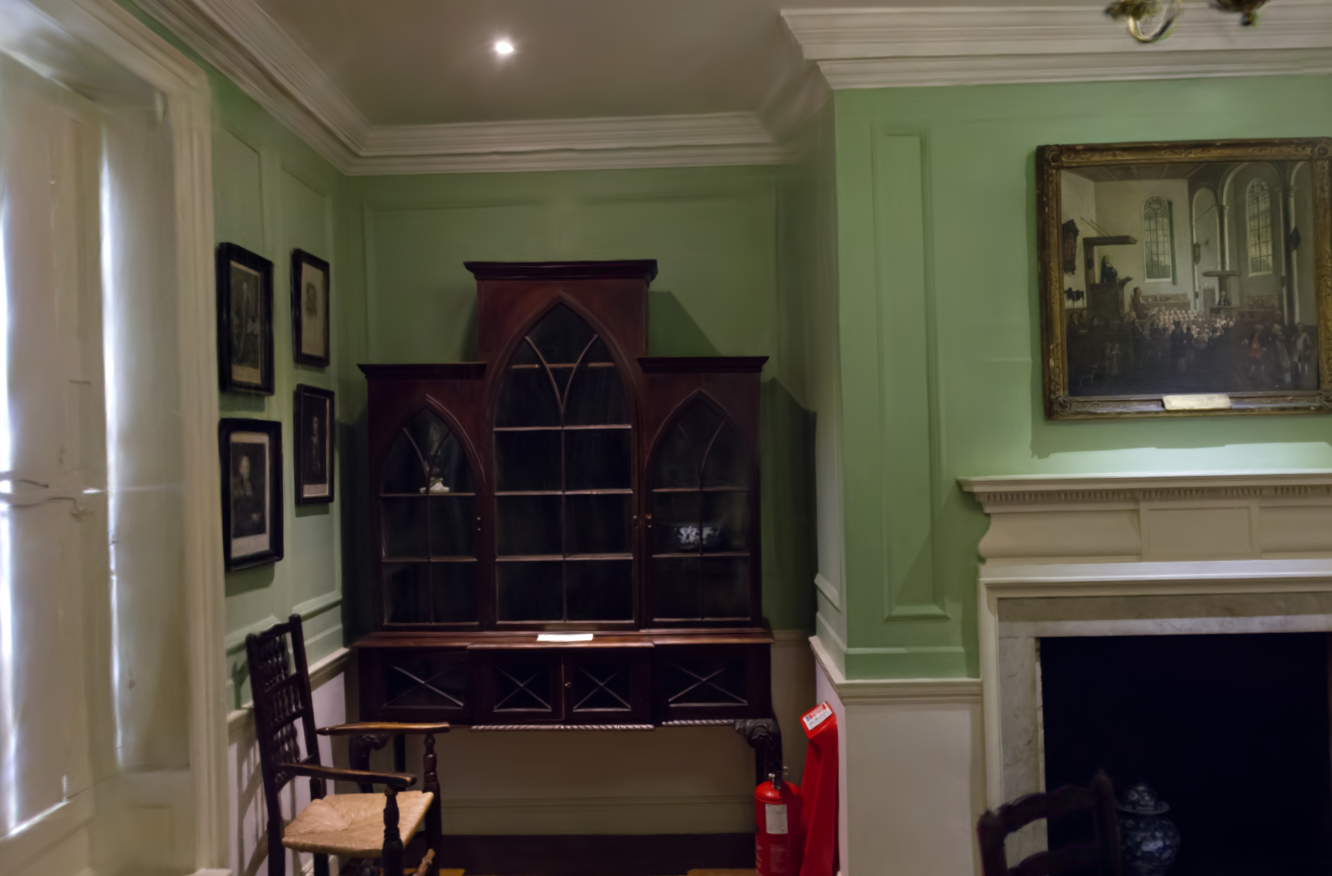
\includegraphics[width=0.235\textwidth]{comparison_figures/view_04_3DGS.png} &
        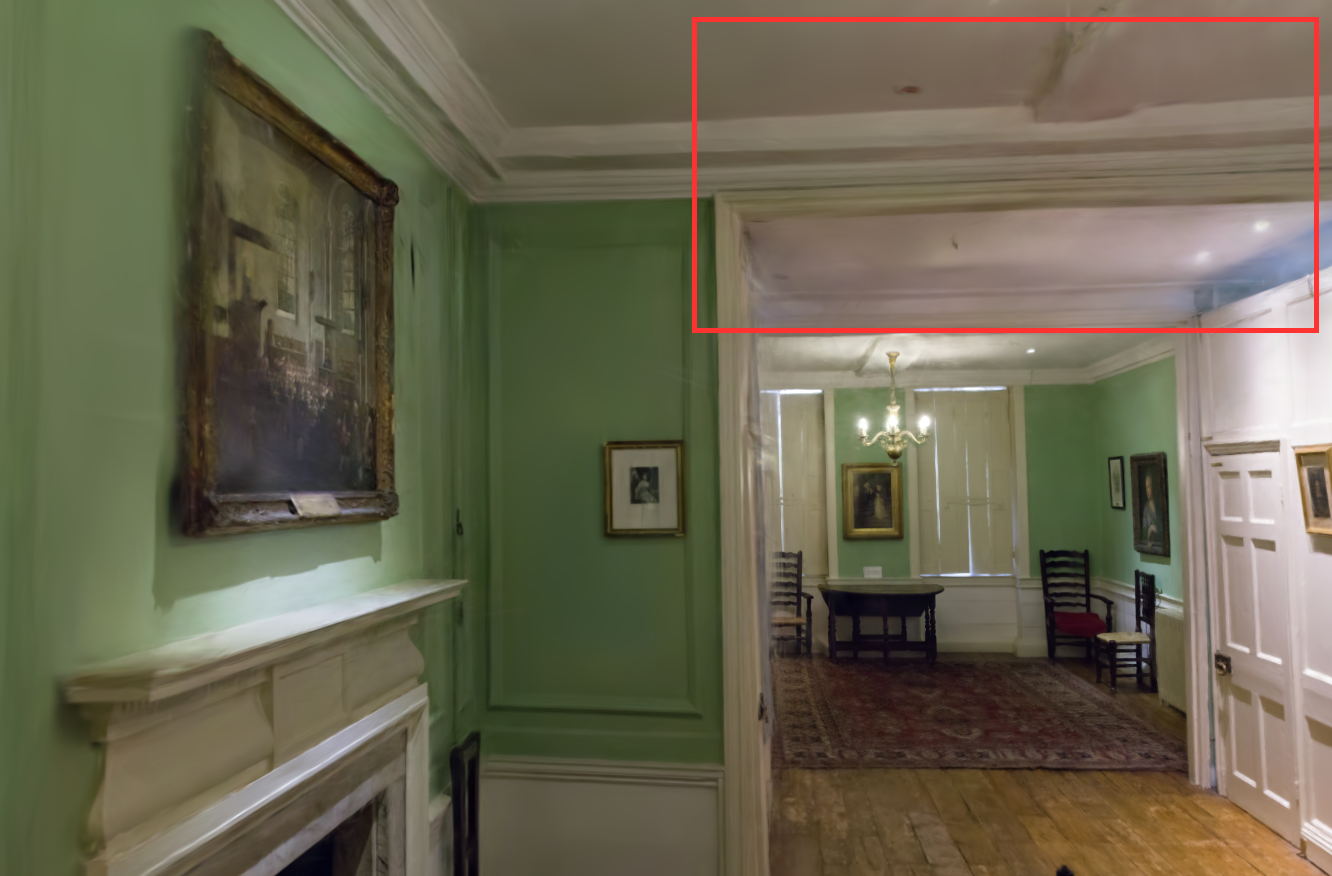
\includegraphics[width=0.235\textwidth]{comparison_figures/view_06_3DGS_rect.png} \\
        \multicolumn{4}{c}{\small\textbf{(b) 3D Gaussian Splatting} — 740 MB} \\[4pt]
        % GeoGaussian row
        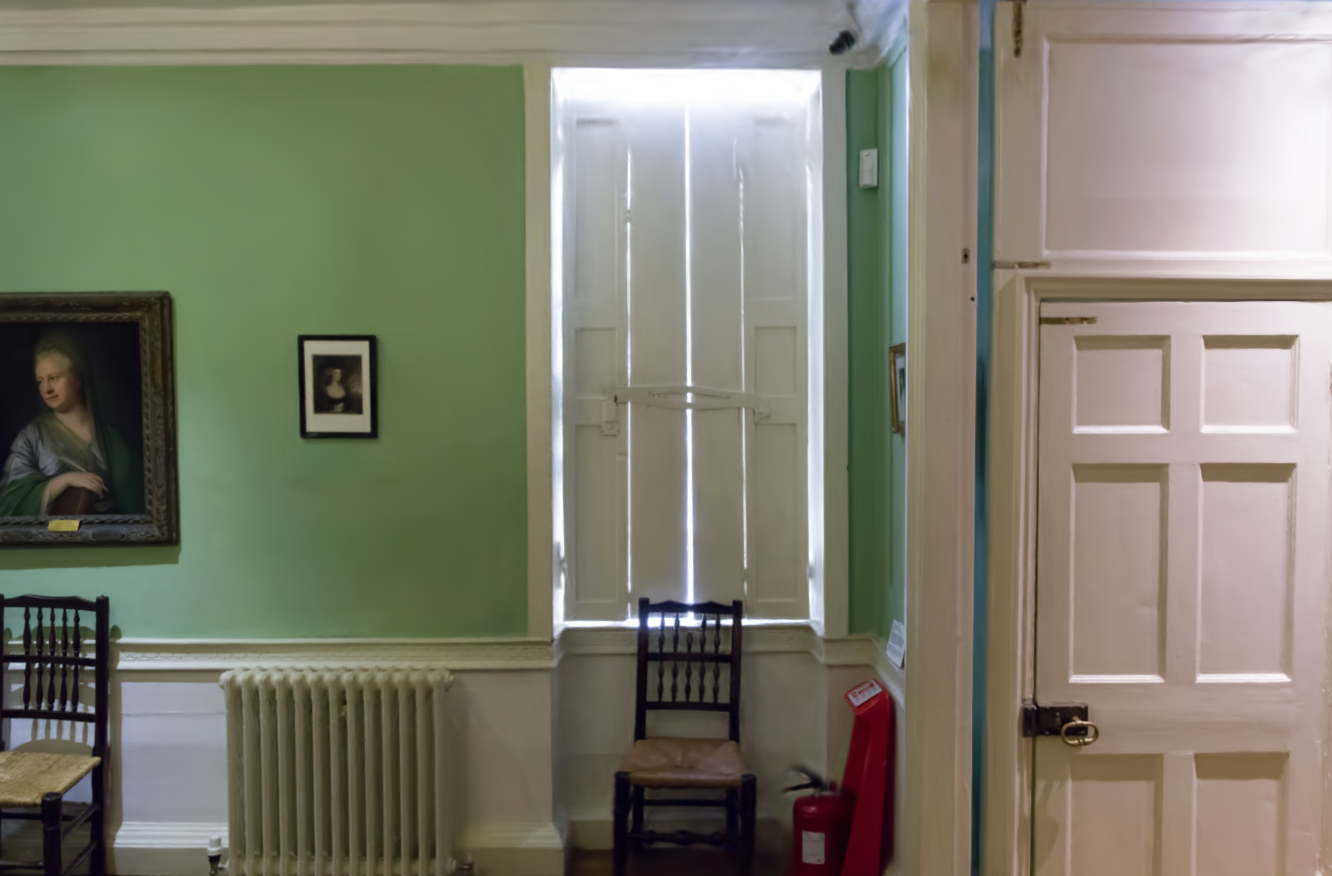
\includegraphics[width=0.235\textwidth]{comparison_figures/view_01_GeoGaussian.png} &
        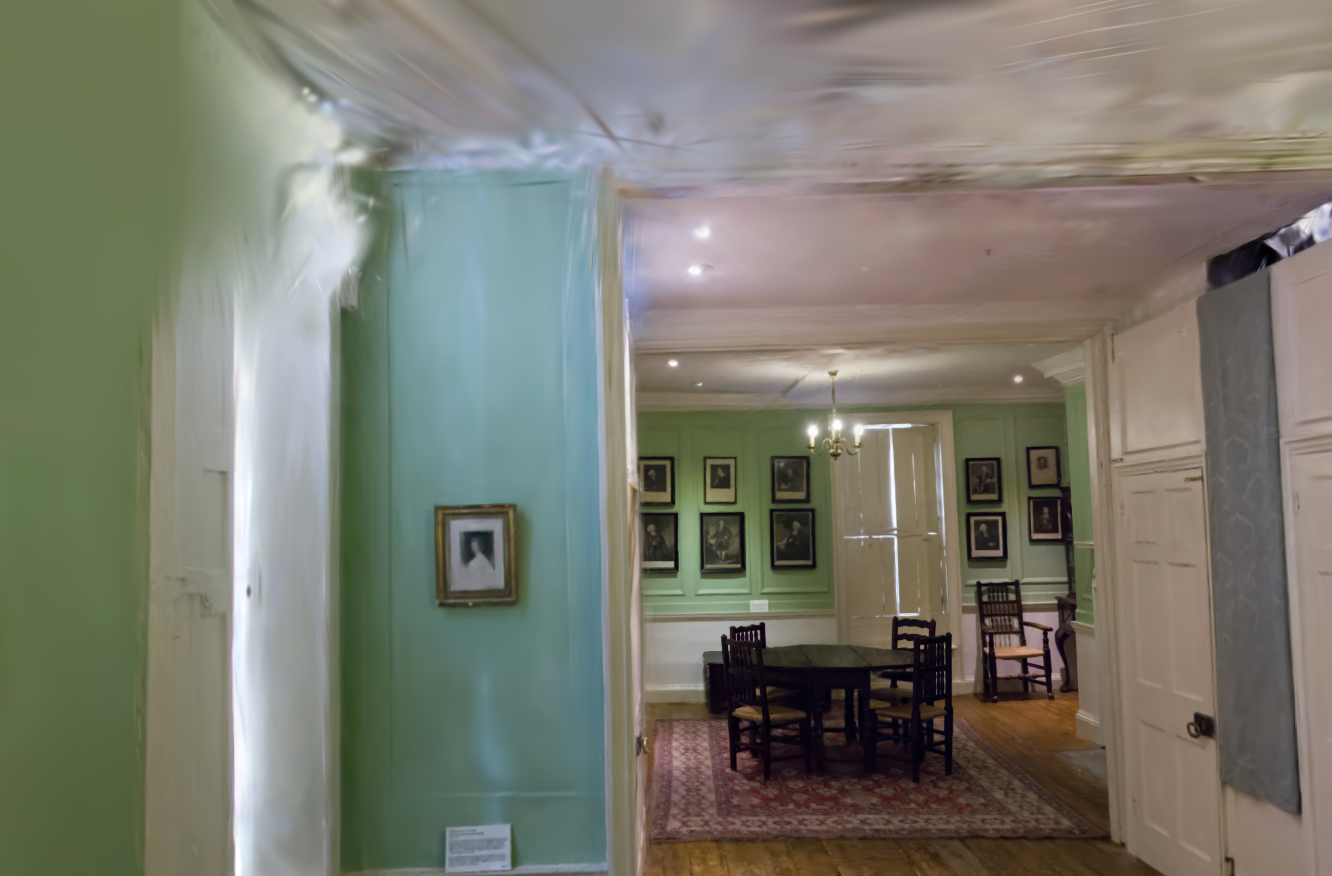
\includegraphics[width=0.235\textwidth]{comparison_figures/view_03_GeoGaussian.png} &
        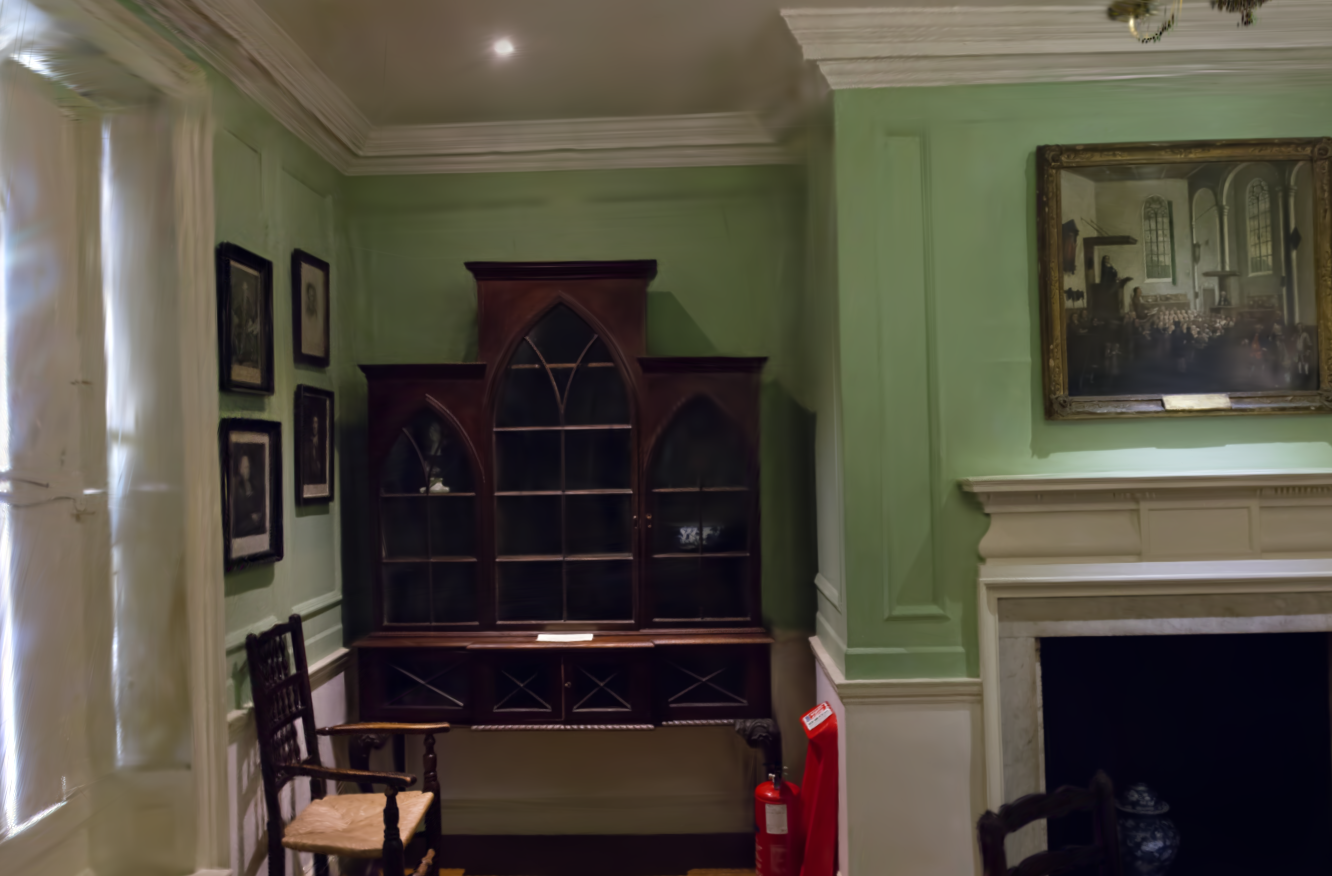
\includegraphics[width=0.235\textwidth]{comparison_figures/view_04_GeoGaussian.png} &
        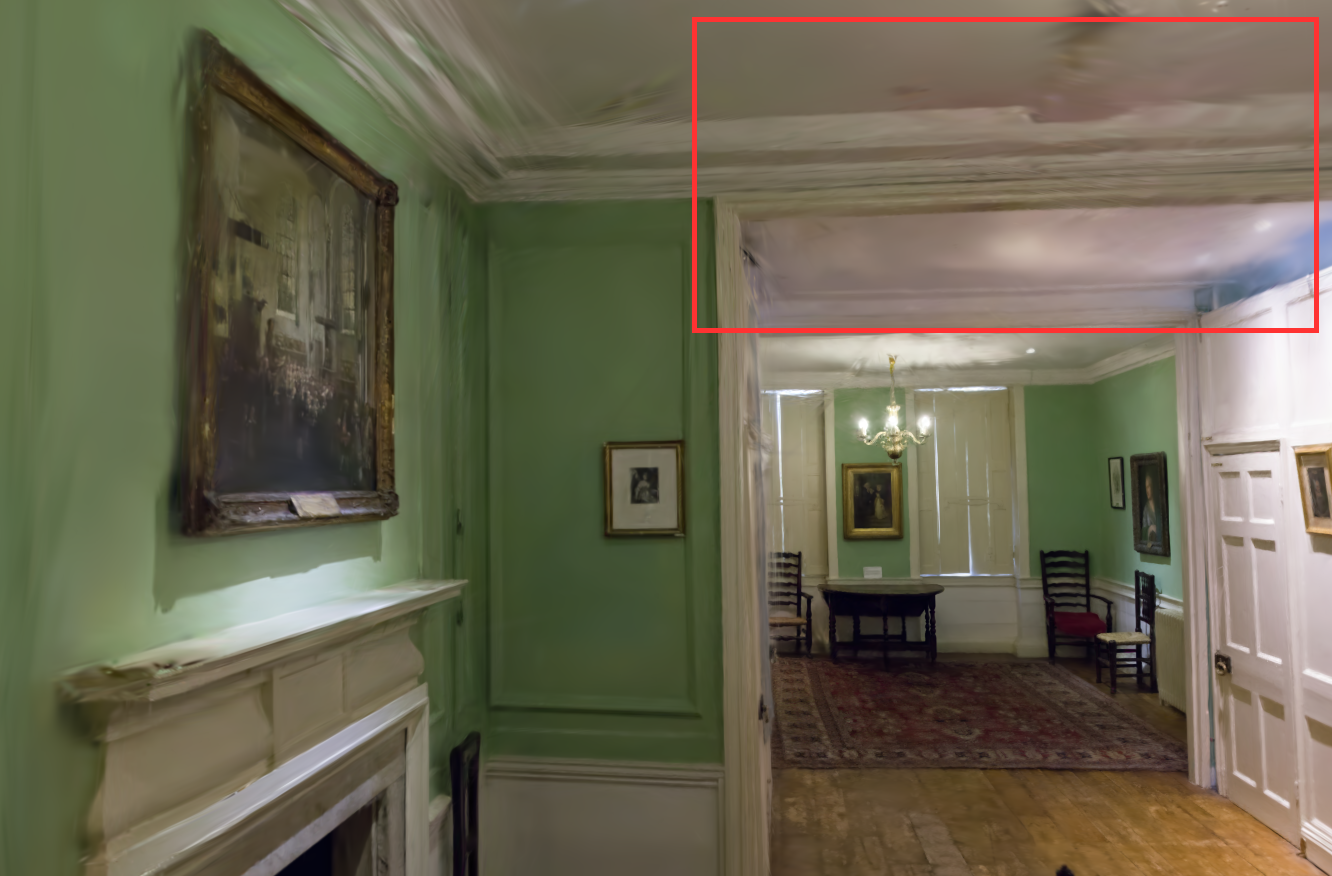
\includegraphics[width=0.235\textwidth]{comparison_figures/view_06_GeoGaussian_rect.png} \\
        \multicolumn{4}{c}{\small\textbf{(c) GeoGaussian} — 281 MB} \\[4pt]
        % PlanarGS row
        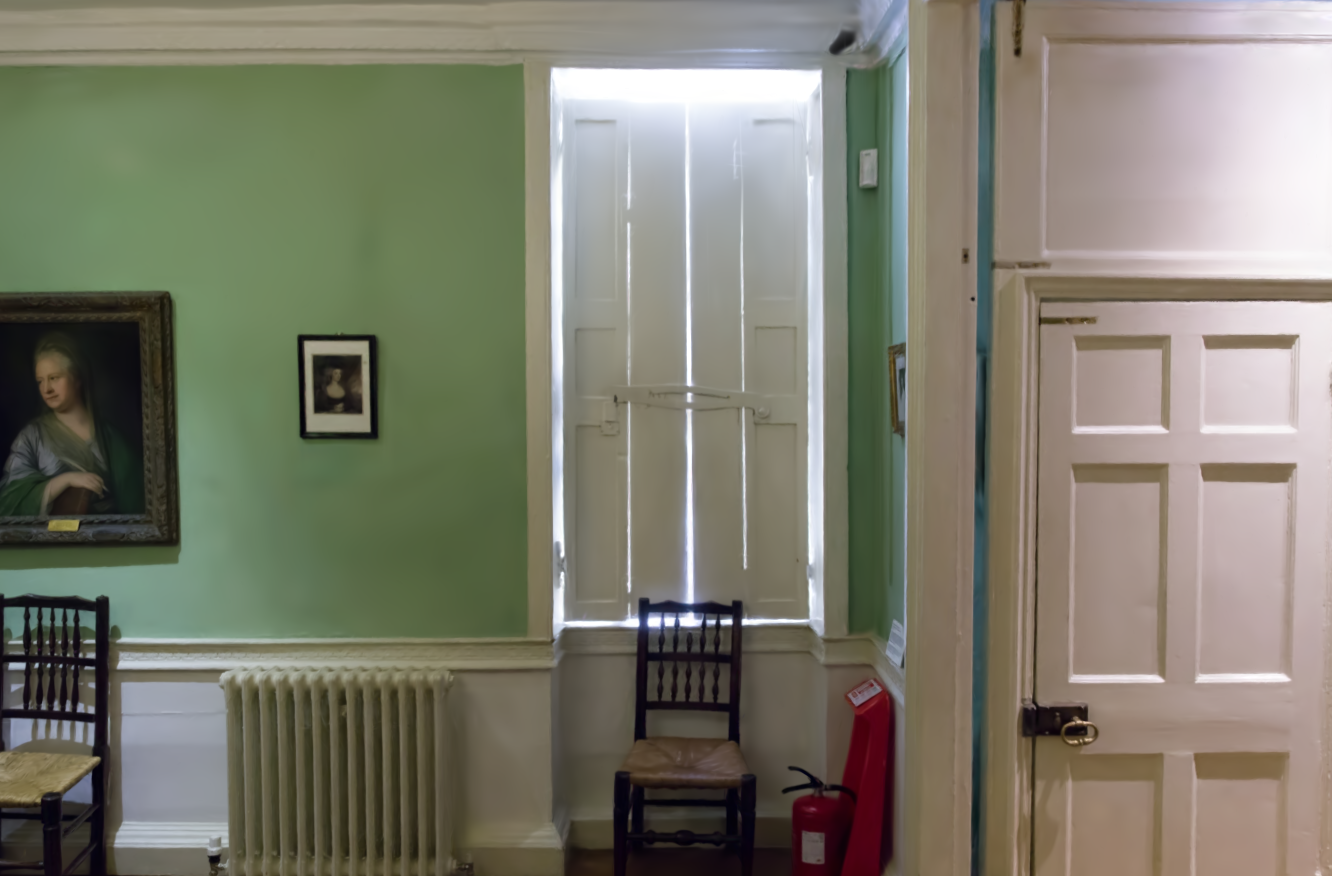
\includegraphics[width=0.235\textwidth]{comparison_figures/view_01_PlanarGS.png} &
        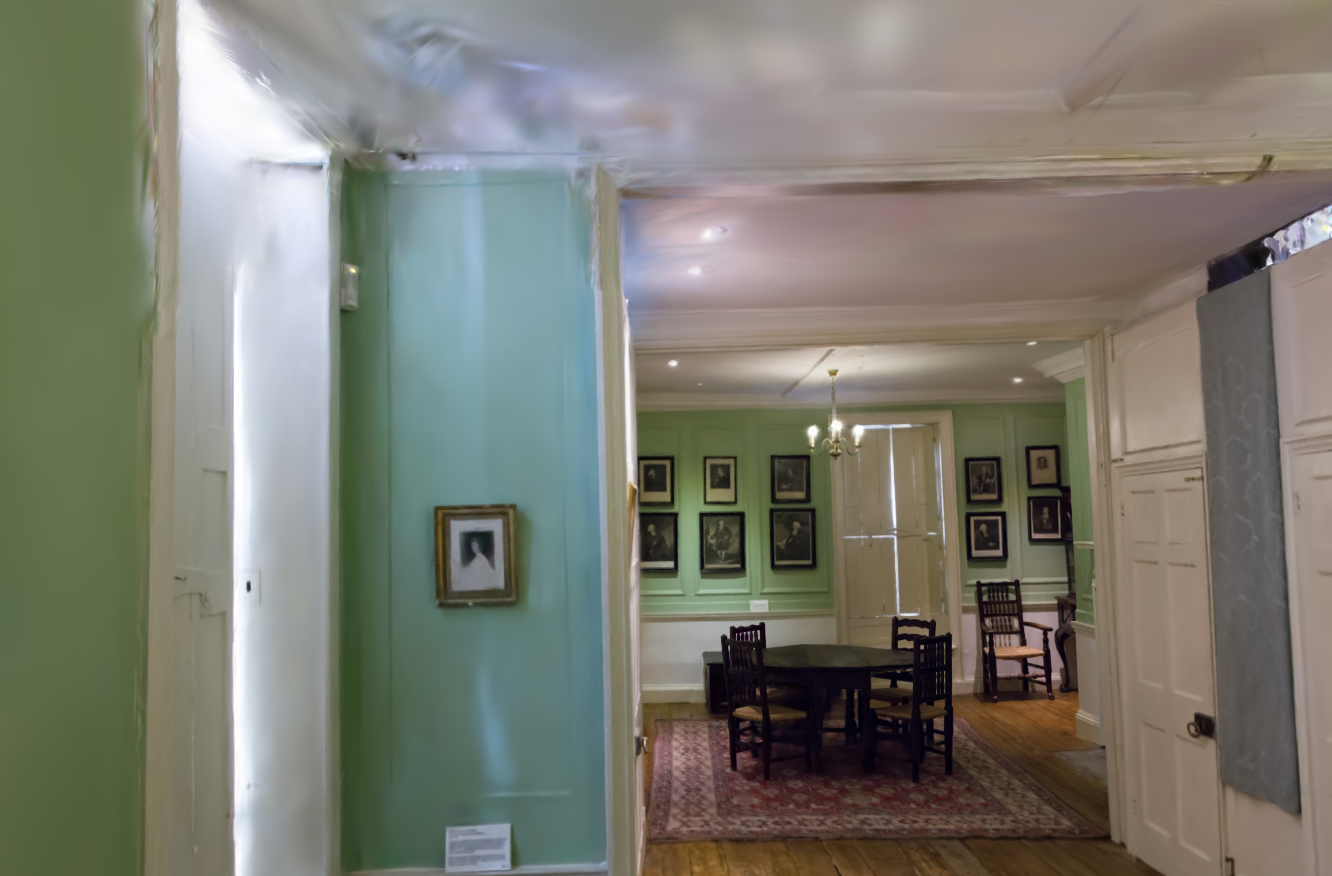
\includegraphics[width=0.235\textwidth]{comparison_figures/view_03_PlanarGS.png} &
        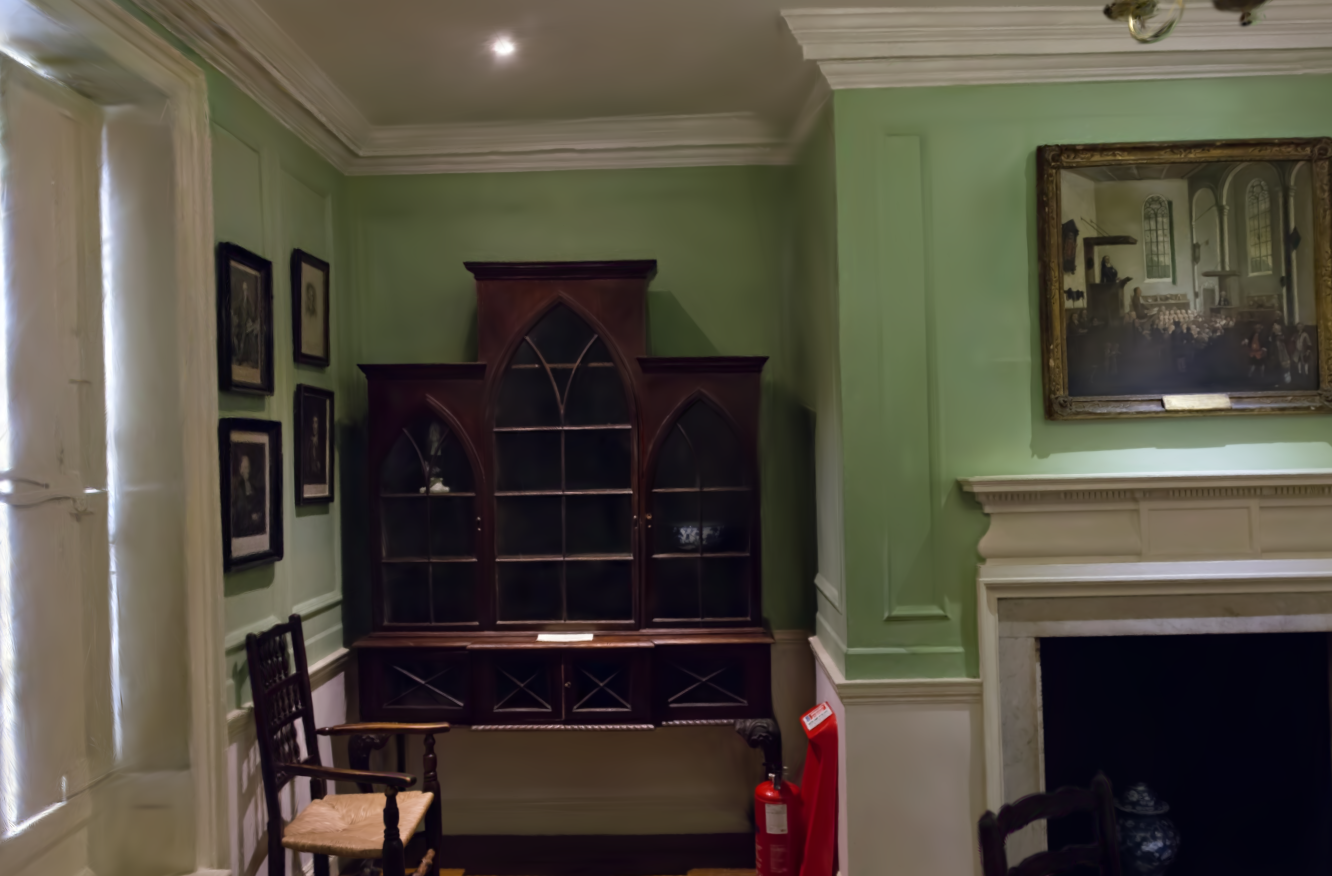
\includegraphics[width=0.235\textwidth]{comparison_figures/view_04_PlanarGS.png} &
        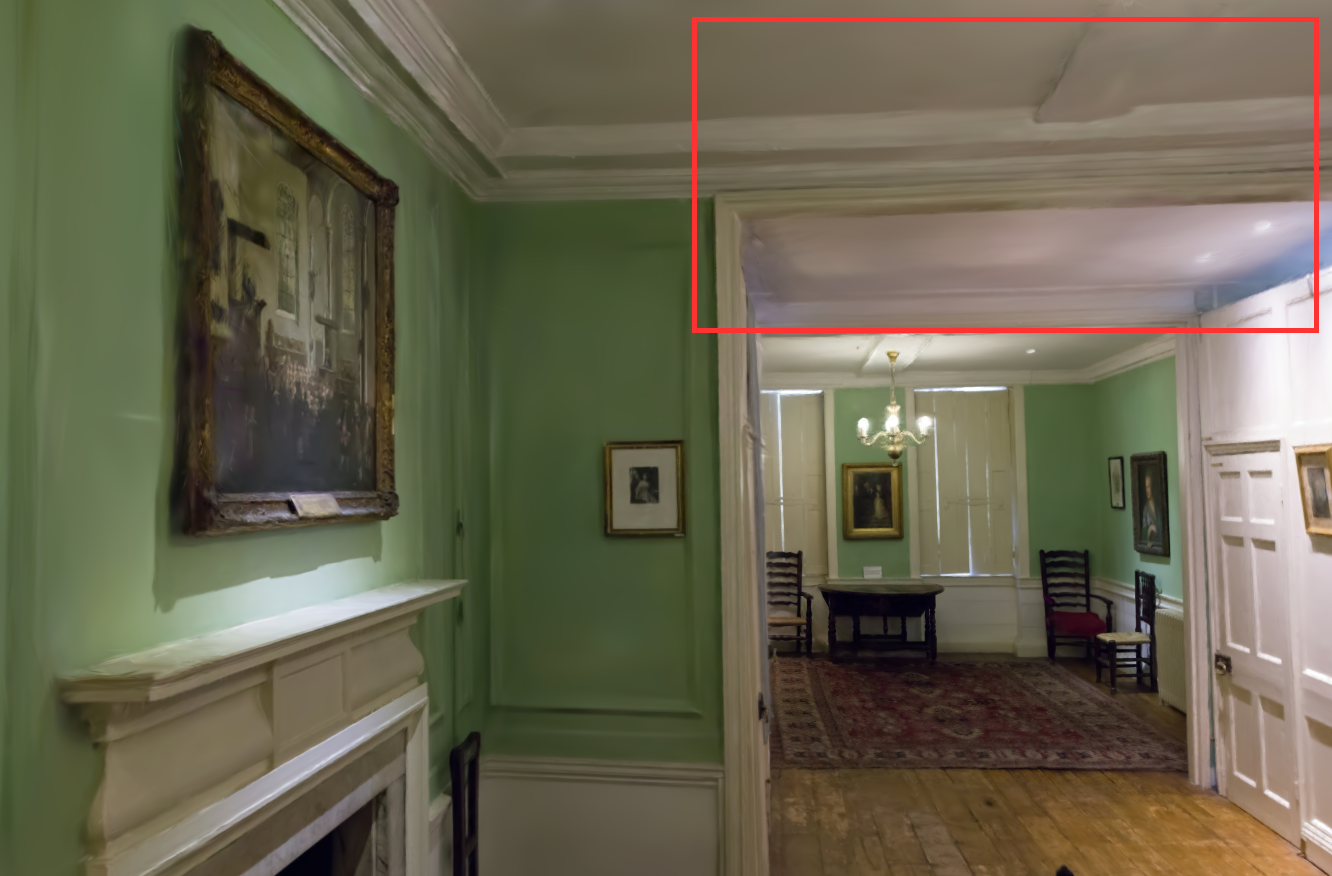
\includegraphics[width=0.235\textwidth]{comparison_figures/view_06_PlanarGS_rect.png} \\
        \multicolumn{4}{c}{\small\textbf{(d) PlanarGS} — 410 MB} \\[4pt]
        % Ours row
        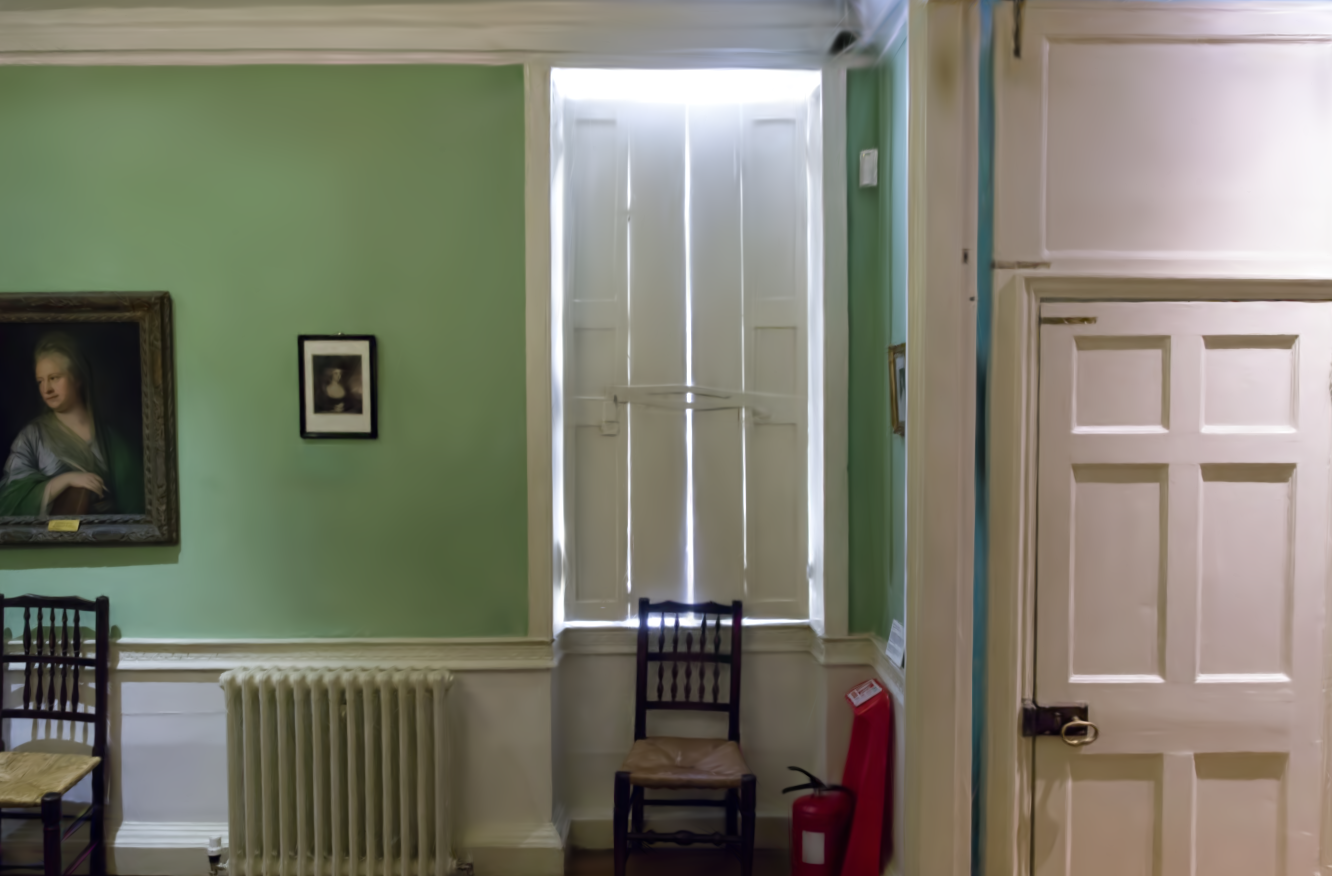
\includegraphics[width=0.235\textwidth]{comparison_figures/view_01_PlanarGS_Opus_new.png} &
        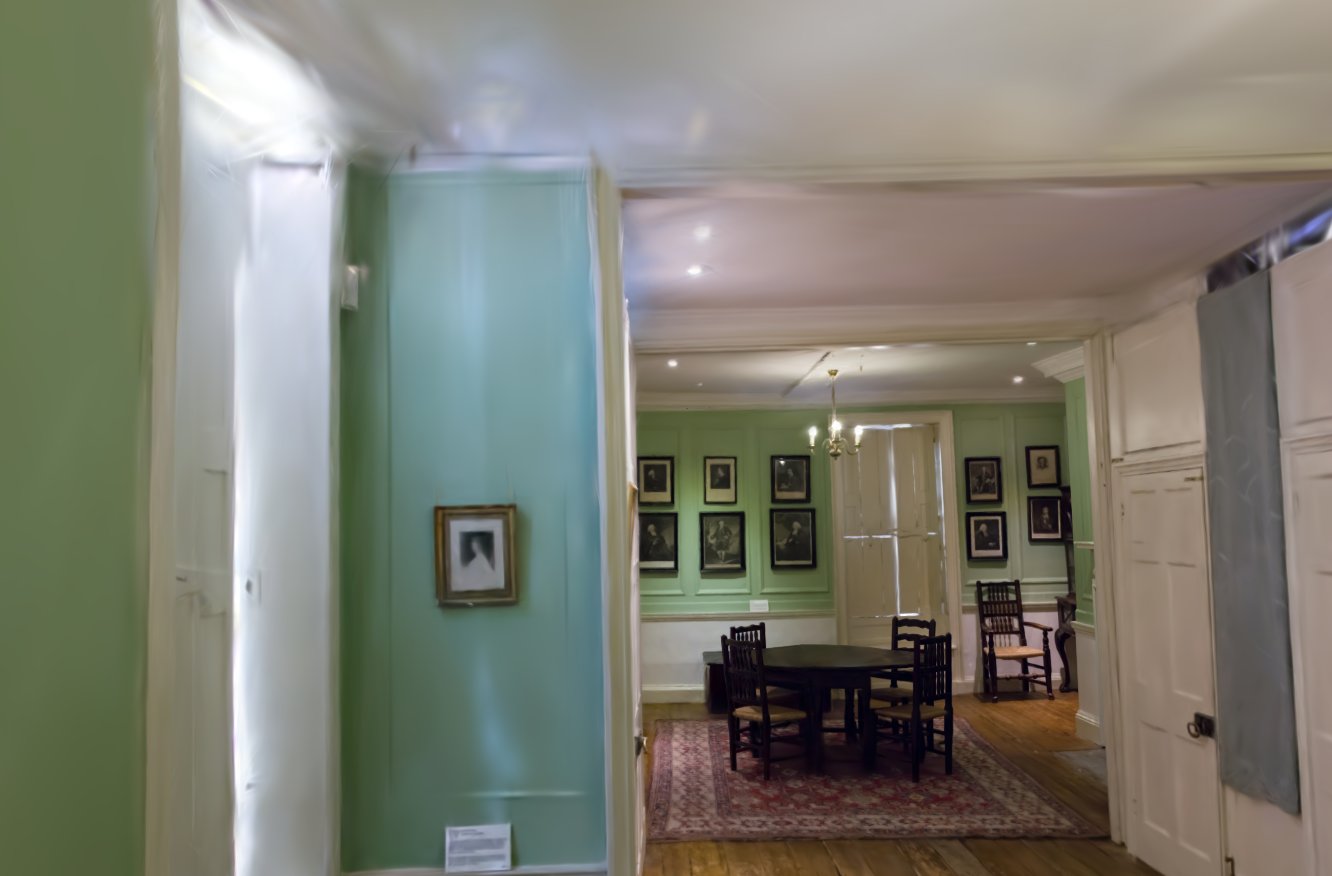
\includegraphics[width=0.235\textwidth]{comparison_figures/view_03_PlanarGS_Opus_new.png} &
        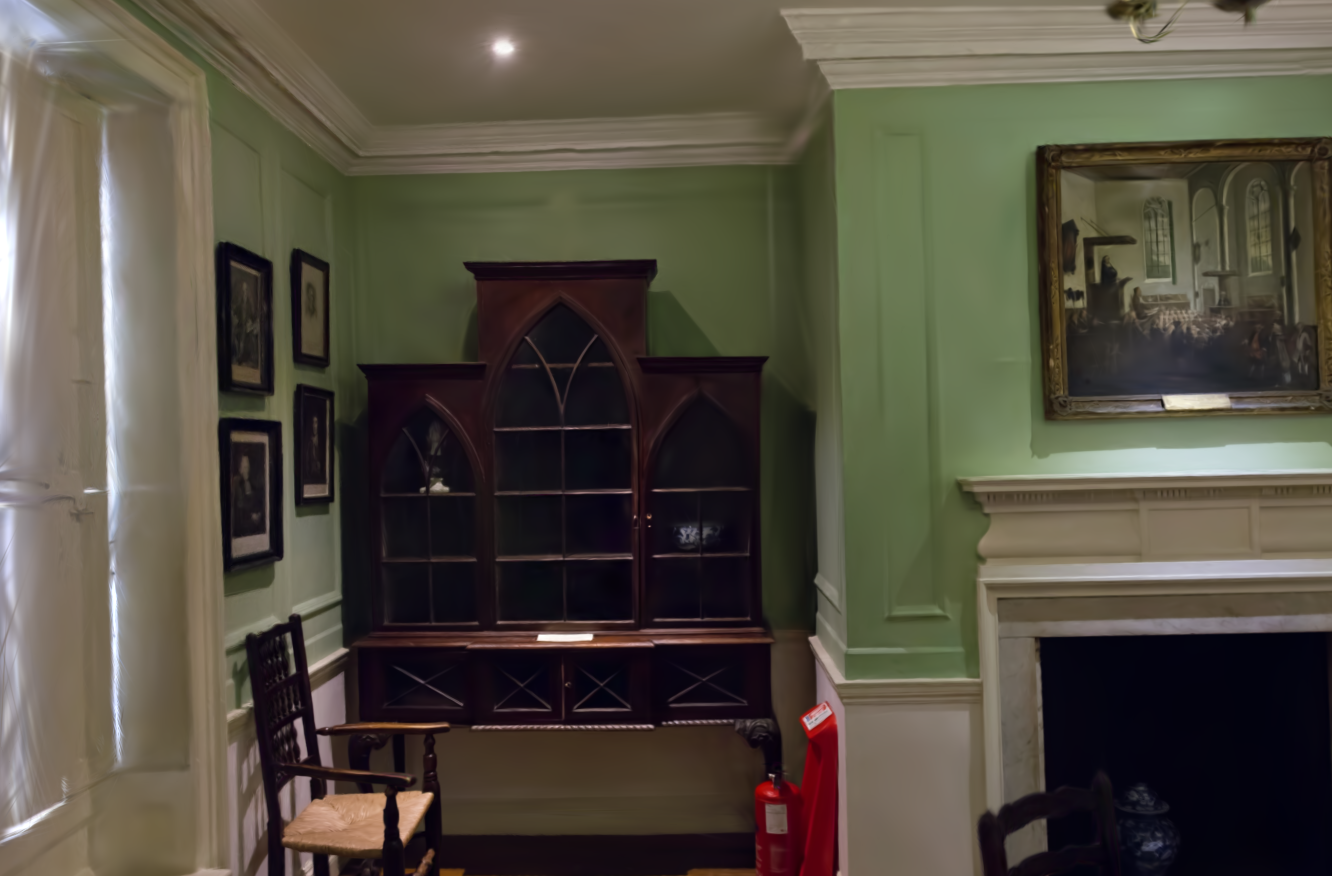
\includegraphics[width=0.235\textwidth]{comparison_figures/view_04_PlanarGS_Opus_new.png} &
        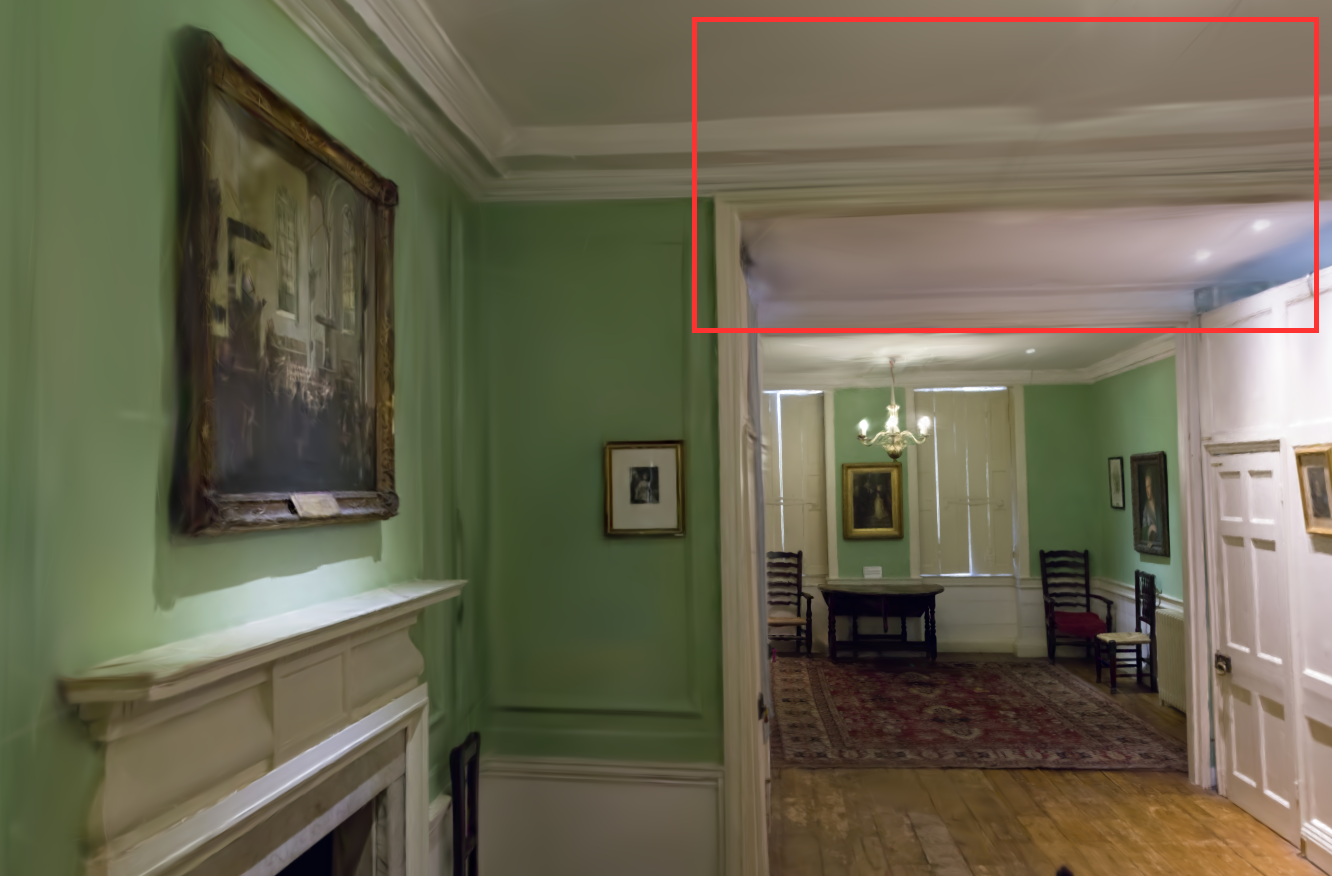
\includegraphics[width=0.235\textwidth]{comparison_figures/view_06_Ours_rect.png} \\
        \multicolumn{4}{c}{\small\textbf{(e) Ours (PlanarGS + edge-aware)} — 222 MB} \\
    \end{tabular}

    \caption{Qualitative comparison on DrJohnson across four viewpoints. Model sizes are PLY file sizes at 30{,}000 iterations. See Table~\ref{tab:method_comparison} for quantitative metrics.}
    \label{fig:qualitative_comparison}
\end{figure}

Visual quality across methods appears subjectively similar in standard RGB renders, despite dramatic differences in model size. Baseline 3D-GS requires 740~MB; GeoGaussian reduces this to 281~MB (62\% smaller) through geometry-guided initialization; PlanarGS reaches 410~MB (45\% smaller) via planar primitive flattening; and our method achieves 222~MB (70\% smaller) by applying edge-aware adaptive densification on top of the PlanarGS backbone. The size reduction stems from concentrating primitives near structural boundaries, regularizing flat surfaces to suppress unnecessary densification, and selecting only complementary priors to avoid conflicting gradients. Taken together, these choices yield a compact representation without a perceptible drop in rendering quality.

\subsection{Structural Quality and Artifact Reduction}

Qualitative analysis reveals that configurations incorporating planarity and edge-aware constraints produce visibly cleaner reconstructions near planar boundaries. Standard Gaussian Splatting methods tend to produce floating artifacts and inconsistent depth discontinuities at object edges, whereas geometry-aware regularization enforces coherent surfaces and sharp transitions.

These improvements are particularly evident in regions with weak texture, where photometric supervision alone is insufficient to constrain geometry. Configurations with planarity and edge-aware priors produce visibly sharper planar boundaries and fewer floating artifacts compared to the baseline.

\subsection{Summary of Findings}

The comprehensive ablation study addresses the core research question — \textit{Can geometric priors enable compact 3D scene representations without sacrificing visual quality?} — and the answer is yes, but only when priors are chosen selectively.

Edge-aware adaptive densification is the most practically valuable component: it reduces model size by 30--32\% with a PSNR drop of only 0.3--0.6~dB, a trade-off that is imperceptible under normal viewing conditions and directly relevant for memory-constrained deployment. Planarity and depth constraints further improve Gaussian utilization by 5--8\%, discouraging over-densification on flat surfaces. Crucially, the full configuration with all five priors enabled (27.63~dB) is outperformed by simpler combinations such as \textit{depths\_planarity} (27.92~dB), confirming that conflicting geometric constraints can destabilize optimization — more regularization is not always better.

Normal priors exhibit clear redundancy with depth and planarity in structured indoor environments, providing diminishing returns when stronger structural cues are already active. Mesh-based regularization is the most expensive prior (4$\times$ training time increase) with the smallest rendering quality gain, and should only be included when downstream mesh extraction is explicitly required. Integrating geometry-aware regularization thus improves both quality and compactness simultaneously, but the design choice of which priors to combine is as important as the choice to use priors at all.